% !TeX program = pdflatex
% =============================================================================
% Arbeitsblatt: Beschleunigung (nicht bewertet, Übungsmaterial für den Unterricht)
% Kantonsschule KFR – Physik, 4. Klasse, 1. HS, Mechanik
%
% Kopiert aus vorlagen/arbeitsblatt-vorlage.tex und um dieselben
% Farb-/Boxdefinitionen ergänzt wie s-t-diagramm-arbeitsblatt.tex /
% v-t-diagramm-arbeitsblatt.tex (selbes Thema-Cluster, direkt anschliessende
% Lektion) -- Templates sind selbstständig/nicht DRY, siehe CLAUDE.md.
%
% Stand: Lernziele, Einstieg, Theorie und Aufgaben fertig (Reihenfolge =
% Dokumentreihenfolge, siehe Kommentar vor der Lernziele-infobox unten,
% entspricht hier zufällig auch der Reihenfolge aus lernziele.md, da
% Backward-Design-Reihenfolge und pädagogisch sinnvolle Dokumentreihenfolge
% hier bereits übereinstimmen).
% =============================================================================
\documentclass[addpoints,11pt,a4paper]{exam}

\usepackage[T1]{fontenc}
\usepackage[utf8]{inputenc}
\usepackage[ngerman]{babel}
\usepackage{lmodern}
\usepackage[a4paper,margin=2.2cm,headheight=14pt]{geometry}
\usepackage{amsmath}
\usepackage{siunitx}
% Hausstil: zusammengesetzte Einheiten immer als echter Bruch (\frac), nicht
% als Inline-Schrägstrich oder \tfrac -- gilt global für jedes \si/\SI.
\sisetup{per-mode=fraction,fraction-command=\frac}
\usepackage{array,booktabs,tabularx,multirow}
\usepackage{enumitem}
\usepackage{graphicx}
\usepackage{xcolor}
\usepackage{colortbl}
\usepackage{tikz}
\usepackage{physics}
\usepackage{circuitikz}
\usepackage[most]{tcolorbox}
\usepackage{lastpage}
\usepackage{needspace}
\usepackage{hyperref}

\usetikzlibrary{arrows.meta,calc,angles,quotes}

\setlength{\parindent}{0pt}
\setlength{\parskip}{0.45em}

% -----------------------------
% Farben (Corporate-Farbschema Physik KFR)
% -----------------------------
\definecolor{titleblue}{HTML}{183A6B}
\definecolor{accentblue}{HTML}{2E6F9E}
\definecolor{lightblue}{HTML}{EAF4FB}
\definecolor{verylightblue}{HTML}{F7FBFE}
\definecolor{lightgray}{HTML}{F4F6F8}
\definecolor{darkgray}{HTML}{4A4A4A}
% Für Diagramme mit zwei verschiedenen Funktionen/Linien: titleblue (dunkles
% Blau) + accentorange (Orange) sind weit genug auseinander (auch in
% Graustufen/für Farbenblinde unterscheidbar), im Gegensatz zu
% titleblue+accentblue, die beide Blautöne sind.
\definecolor{accentorange}{HTML}{D9720C}
% Für Diagramme mit DREI Linien: dritte Farbe nötig, die sich sowohl von
% titleblue als auch von accentorange klar unterscheidet -- auch in
% Graustufen/für Farbenblinde. Violett liegt weit genug von Blau und Orange
% entfernt, um als dritte Linie eindeutig unterscheidbar zu bleiben.
\definecolor{accentpurple}{HTML}{7B2D8E}
% Kein eigenes Grün/Petrol mehr für Theorie-/Gruppenarbeit-Box: dieses
% Arbeitsblatt übernimmt das Boxen-Layout von institutionen/UZH-Praktikum-I
% (siehe dortiges CLAUDE.md, "Boxen-Layout") -- Lernziele/Einleitung/Theorie/
% Aufgaben werden ungerahmt, nur formelbox/hinweisbox/answerbox bleiben
% farbig. Bewusste Abweichung vom sonstigen KFR-Hausstil nur in dieser Datei.

% Links (hyperref): farblich ans Corporate-Farbschema angeglichen, für den
% Simulations-Link bei der PhET-Übung.
\hypersetup{
  colorlinks=true,
  urlcolor=accentblue,
  linkcolor=accentblue,
  pdftitle={Arbeitsblatt: Beschleunigung},
  pdfauthor={Loris Keller}
}

% -----------------------------
% Spaltentypen
% -----------------------------
\newcolumntype{Y}{>{\centering\arraybackslash}X}
\newcolumntype{P}[1]{>{\raggedright\arraybackslash}p{#1}}

% -----------------------------
% Boxen
% -----------------------------
\tcbset{before skip=10pt, after skip=10pt}
\newtcolorbox{titlebox}{
  enhanced,
  colback=titleblue,
  colframe=titleblue,
  boxrule=0pt,
  arc=3mm,
  left=3mm,right=3mm,top=3mm,bottom=3mm
}

% infobox/theoriebox/beispielbox: ungerahmter Fliesstext statt farbiger Box
% (Layout wie Praktikum I), Titel wird -- wo vorhanden -- manuell/über das
% optionale Argument fett gesetzt.
% Regel bleibt unverändert: hervorgehobene/definierte Begriffe INNERHALB
% einer theoriebox immer mit \textbf{\emph{...}} setzen (fett UND kursiv),
% nicht mit blossem \emph{...} -- damit Fachbegriffe beim Durchlesen der
% Theorie sofort auffallen. Ausserhalb von theoriebox (beispielbox,
% Aufgabentext, ...) bleibt \emph{...} allein korrekt.
\newenvironment{infobox}{%
  \par\addvspace{10pt}\noindent
}{%
  \par\addvspace{10pt}
}

\newenvironment{theoriebox}[1][Theorie]{%
  \par\addvspace{10pt}\noindent\textbf{#1}\par\smallskip\noindent
}{%
  \par\addvspace{10pt}
}

% taskbox/groupbox bleiben technisch tcolorboxen (nur unsichtbar gemacht:
% keine Farbe/kein Rahmen/kein Padding), weil sie innerhalb der
% exam-Klasse questions-Liste vor dem ersten \question stehen können
% (Bild/Fliesstext) -- eine reine \newenvironment löst dort "Something's
% wrong--perhaps a missing \item", sobald z.B. ein \begin{center} vor dem
% ersten \item der Aussenliste steht.
% exam.cls rückt die questions-Liste um die Breite von "10." (plus
% \labelsep) ein (Platz für die Nummerierung); ohne Korrektur würde der
% Inhalt von taskbox/groupbox (Diagramme, Fliesstext) deshalb sichtbar
% weiter eingerückt erscheinen als der Inhalt von infobox/theoriebox/
% beispielbox (die ausserhalb von questions stehen und deshalb bereits die
% volle Randbreite nutzen) -- gleicher Randabstand im ganzen Dokument, auch
% bei den Übungen.
\newlength{\aufgabenindent}
\settowidth{\aufgabenindent}{10.\hskip\labelsep}
\newtcolorbox{taskbox}[1][]{
  enhanced, breakable,
  colback=white, colframe=white, boxrule=0pt,
  left=0mm,right=0mm,top=0mm,bottom=0mm,
  before skip=10pt, after skip=10pt,
  enlarge left by=-\aufgabenindent,
  width=\textwidth,
  before upper={%
    \def\tmpboxtitle{#1}%
    \ifx\tmpboxtitle\empty\else\noindent\textbf{#1}\par\smallskip\fi
  }
}

\newenvironment{beispielbox}[1][Beispiel]{%
  \par\addvspace{10pt}\noindent\textbf{#1}\par\smallskip\noindent
}{%
  \par\addvspace{10pt}
}

% groupbox: Regel bleibt unverändert -- JEDE Aufgabe, bei der
% Schülerinnen/Schüler zu zweit oder in einer Gruppe zusammenarbeiten,
% bekommt diese Box statt der taskbox (in diesem Arbeitsblatt aktuell nicht
% verwendet, aber weiterhin definiert für künftige Gruppenaufgaben).
\newtcolorbox{groupbox}[1][Gruppenarbeit]{
  enhanced, breakable,
  colback=white, colframe=white, boxrule=0pt,
  left=0mm,right=0mm,top=0mm,bottom=0mm,
  before skip=10pt, after skip=10pt,
  enlarge left by=-\aufgabenindent,
  width=\textwidth,
  before upper={\noindent\textbf{#1}\par\smallskip}
}

% hinweisbox: bleibt farbig (Orange, accentorange) -- wichtige
% Klarstellungen, die über eine normale Inline-Bemerkung (wie das
% bestehende "\textbf{Wichtig:}" innerhalb einer theoriebox) hinausgehen,
% sollen trotz des sonst ungerahmten Layouts weiterhin auffallen.
\definecolor{lightorange}{HTML}{FCEEE0}
\newtcolorbox{hinweisbox}[1][Hinweis]{
  enhanced,
  breakable,
  colback=lightorange,
  colframe=accentorange,
  title={#1},
  fonttitle=\bfseries,
  boxrule=0.7pt,
  arc=2mm,
  left=5mm,right=5mm,top=2mm,bottom=2mm
}

% formelbox: eigene Farbe (Violett, accentpurple, wiederverwendet aus den
% Tangente-/Diagrammfarben), damit die zentralen Formeln dieser Einheit auf
% einen Blick auffindbar bleiben, auch wenn Theorie/Aufgaben sonst
% ungerahmt sind.
\definecolor{lightpurple}{HTML}{F3EAF7}
\newtcolorbox{formelbox}[1][Merksatz]{
  enhanced,
  breakable,
  colback=lightpurple,
  colframe=accentpurple,
  title={#1},
  fonttitle=\bfseries,
  boxrule=0.9pt,
  arc=2mm,
  left=5mm,right=5mm,top=2mm,bottom=2mm
}

\newtcolorbox{answerbox}{
  breakable,
  colback=white,
  colframe=gray!55,
  boxrule=0.5pt,
  arc=1.5mm,
  left=2mm,right=2mm,top=2mm,bottom=2mm
}

% --- Lösungen ein-/ausblenden -----------------------------------------------
% Schülerexemplar (Standard): \noprintanswers
% Lehrer-/Lösungsexemplar:    \printanswers
%\noprintanswers
\printanswers

% --- Punkte bleiben intern, werden aber nicht gedruckt ----------------------
% Arbeitsblätter sind nicht benotet. \question[n]/\part[n] bekommen trotzdem
% eine Punktzahl n -- rein als interner Anhaltspunkt, der 1:1 an
% \Antwortraum{n} weitergereicht wird, um die Antwortraum-Grösse zu
% bestimmen. \pointformat{} (Aufruf, nicht \renewcommand!) unterdrückt die
% von der exam-Klasse sonst automatisch gedruckte Punktanzeige ("(n P.)")
% vollständig, ohne die interne Punktezählung (\numpoints) zu beeinflussen.
\pointformat{}

% --- Lösungsbox auf Deutsch, farblich abgesetzt -----------------------------
\renewcommand{\solutiontitle}{\noindent\color{titleblue}\textbf{Lösung:}\enspace}

% --- Kopf-/Fusszeile: Thema/Titel oben, Seitenzahl unten --------------------
\pagestyle{headandfoot}
\cfoot{\textcolor{darkgray}{Seite \thepage\ von \pageref{LastPage}}}

% --- Kopfzeile: Klasse / Datum / Thema / Titel ------------------------------
% Einheitliches Layout für Arbeitsblatt, Prüfung und Praktikum. Ohne Tabelle:
% Klasse/Datum/Thema/Lehrperson stehen als einfache Textzeile unter dem
% Titel-Banner. Fünftes Argument (Untertitel) ist eine rein optische
% Ergänzung nur für dieses Arbeitsblatt (grössere/kleinere Zeile im
% Titel-Banner) -- die vier Kernangaben Klasse/Datum/Thema/Titel bleiben in
% derselben Reihenfolge/Position wie im Hausstil-Standard, #4 allein (ohne
% Untertitel) bleibt daher auch die knappe Kopfzeilen-/Seitenkopf-Variante.
\newcommand{\Kopfzeile}[5]{%
  \begin{titlebox}
    {\color{white}\sffamily\bfseries\Large #4}\\[3pt]
    {\color{white}\sffamily\normalsize #5}
  \end{titlebox}
  \vspace{0.5em}
  \noindent\textbf{Klasse:}~#1 \hfill \textbf{Datum:}~#2 \hfill \textbf{Thema:}~#3
    \hfill \textbf{Lehrperson:}~Loris Keller
  \vspace{0.8em}
  \lhead{\textcolor{darkgray}{#3}}
  \rhead{\textcolor{darkgray}{#4}}
}

% --- Antwortraum: ca. 2.5 cm Platz pro Punkt, als umrandetes Feld -----------
\newlength{\antwortraumlen}
\newcommand{\Antwortraum}[1]{%
  \pgfmathsetlength{\antwortraumlen}{#1*2.5cm}%
  \begin{answerbox}
    \rule{0pt}{\antwortraumlen}%
  \end{answerbox}%
}

% Werte für Kopfzeile zentral setzen
\newcommand{\Klasse}{4a}
\newcommand{\Datum}{04.09.2026}
\newcommand{\Thema}{Beschleunigung}
\newcommand{\ArbeitsblattTitel}{Arbeitsblatt: Beschleunigung}
\newcommand{\ArbeitsblattUntertitel}{Änderungsrate der Geschwindigkeit}

\begin{document}

\Kopfzeile{\Klasse}{\Datum}{\Thema}{\ArbeitsblattTitel}{\ArbeitsblattUntertitel}

% --- Lernziele: aus lernziele.md (Backward-Design, Stufe 1) übernommen,
% seither an den tatsächlichen Inhalt dieses Arbeitsblatts angepasst -----
% LZ1..LZ4 entsprechen der Reihenfolge, in der die zugehörigen
% Theorieboxen/Übungen im Dokument erscheinen (wie im s-t-Diagramm- und
% v-t-Diagramm-Arbeitsblatt: LZ1 = das im Arbeitsblatt zuerst behandelte
% Lernziel).
% Reihenfolge: LZ1 (Beschleunigung von Geschwindigkeit unterscheiden) ->
% LZ2/LZ3 (Durchschnitts-/Momentanbeschleunigung als Sekante/Tangente im
% v-t-Diagramm, ganz am Ende des Arbeitsblatts behandelt) -> LZ4
% (Vorzeichen der Beschleunigung, auch bei Verzögerung) -> zusätzliches
% Lernziel zur Weg-Formel (siehe unten).
%
% LZ6 (Geschwindigkeit vs. Beschleunigung unterscheiden) entfernt: Dafür
% wurde nie eine eigene Übung geschrieben, und es deckt sich inhaltlich
% auch mit keiner der später ergänzten Aufgaben -- die gedruckten
% Lernziele sollen den tatsächlichen Inhalt abbilden, nicht ungeprüft
% lernziele.md spiegeln. lernziele.md selbst NICHT anpassen (siehe
% Kommentar dort); falls LZ6 künftig doch abgedeckt werden soll, im
% Backward-Design-Dokument nachführen und diese Liste dann neu abgleichen.
%
% Zusätzliches Lernziel (letzter Punkt unten, bewusst ohne LZ-Nummer, da
% nicht Teil von lernziele.md): deckt die Weg-Formel-Herleitung
% (s=1/2at^2 aus der Fläche im v-t-Diagramm, Umstellung nach s=v^2/2a) ab,
% die auf ausdrücklichen Wunsch ergänzt wurde, obwohl lernziele.md diesen
% Stoff explizit der separaten Bewegungsgleichungen-Einheit zuordnet
% (siehe Kommentare weiter unten bei den jeweiligen Boxen).
%
% LZ5 (Beschleunigung am Umkehrpunkt) bewusst NICHT in diesem Arbeitsblatt:
% Umkehrpunkt/Jongleur-Szenario wird zu einem eigenen Thema (eigenes
% künftiges Arbeitsblatt), deshalb hier entfernt statt nur verschoben.
% lernziele.md selbst NICHT anpassen (siehe Kommentar dort), die
% Zuordnung von LZ5 zu einem künftigen Arbeitsblatt bei Bedarf im
% Backward-Design-Dokument nachführen.
\begin{infobox}
\textbf{Lernziele}\\
Am Ende dieser Einheit kann ich \dots
\begin{itemize}[leftmargin=1.2cm,itemsep=0.25em]
  \item den Begriff der Beschleunigung als Änderungsrate der Geschwindigkeit von der Geschwindigkeit selbst unterscheiden. (LZ1)
  \item aus einem v-t-Diagramm die Durchschnittsbeschleunigung zwischen zwei Zeitpunkten als Sekantensteigung berechnen. (LZ2)
  \item an einem markierten Punkt eines v-t-Diagramms die Momentanbeschleunigung qualitativ aus der Tangente abschätzen. (LZ3)
  \item das Vorzeichen einer Beschleunigung relativ zu einem gewählten Koordinatensystem korrekt interpretieren, auch bei Verzögerung. (LZ4)
  \item die Formel für den Weg bei einer Bewegung aus dem Stand ($s=\tfrac12at^2$) aus der Fläche im $v$-$t$-Diagramm herleiten und für Berechnungen von Strecke, Geschwindigkeit oder Beschleunigung anwenden.
\end{itemize}
\end{infobox}

% --- Einstieg: Hook vor der formalen Theorie, Bild aus Bilder/ -------------
\begin{beispielbox}[Einstieg: Der schnellste Beschleuniger der Welt]
\begin{center}
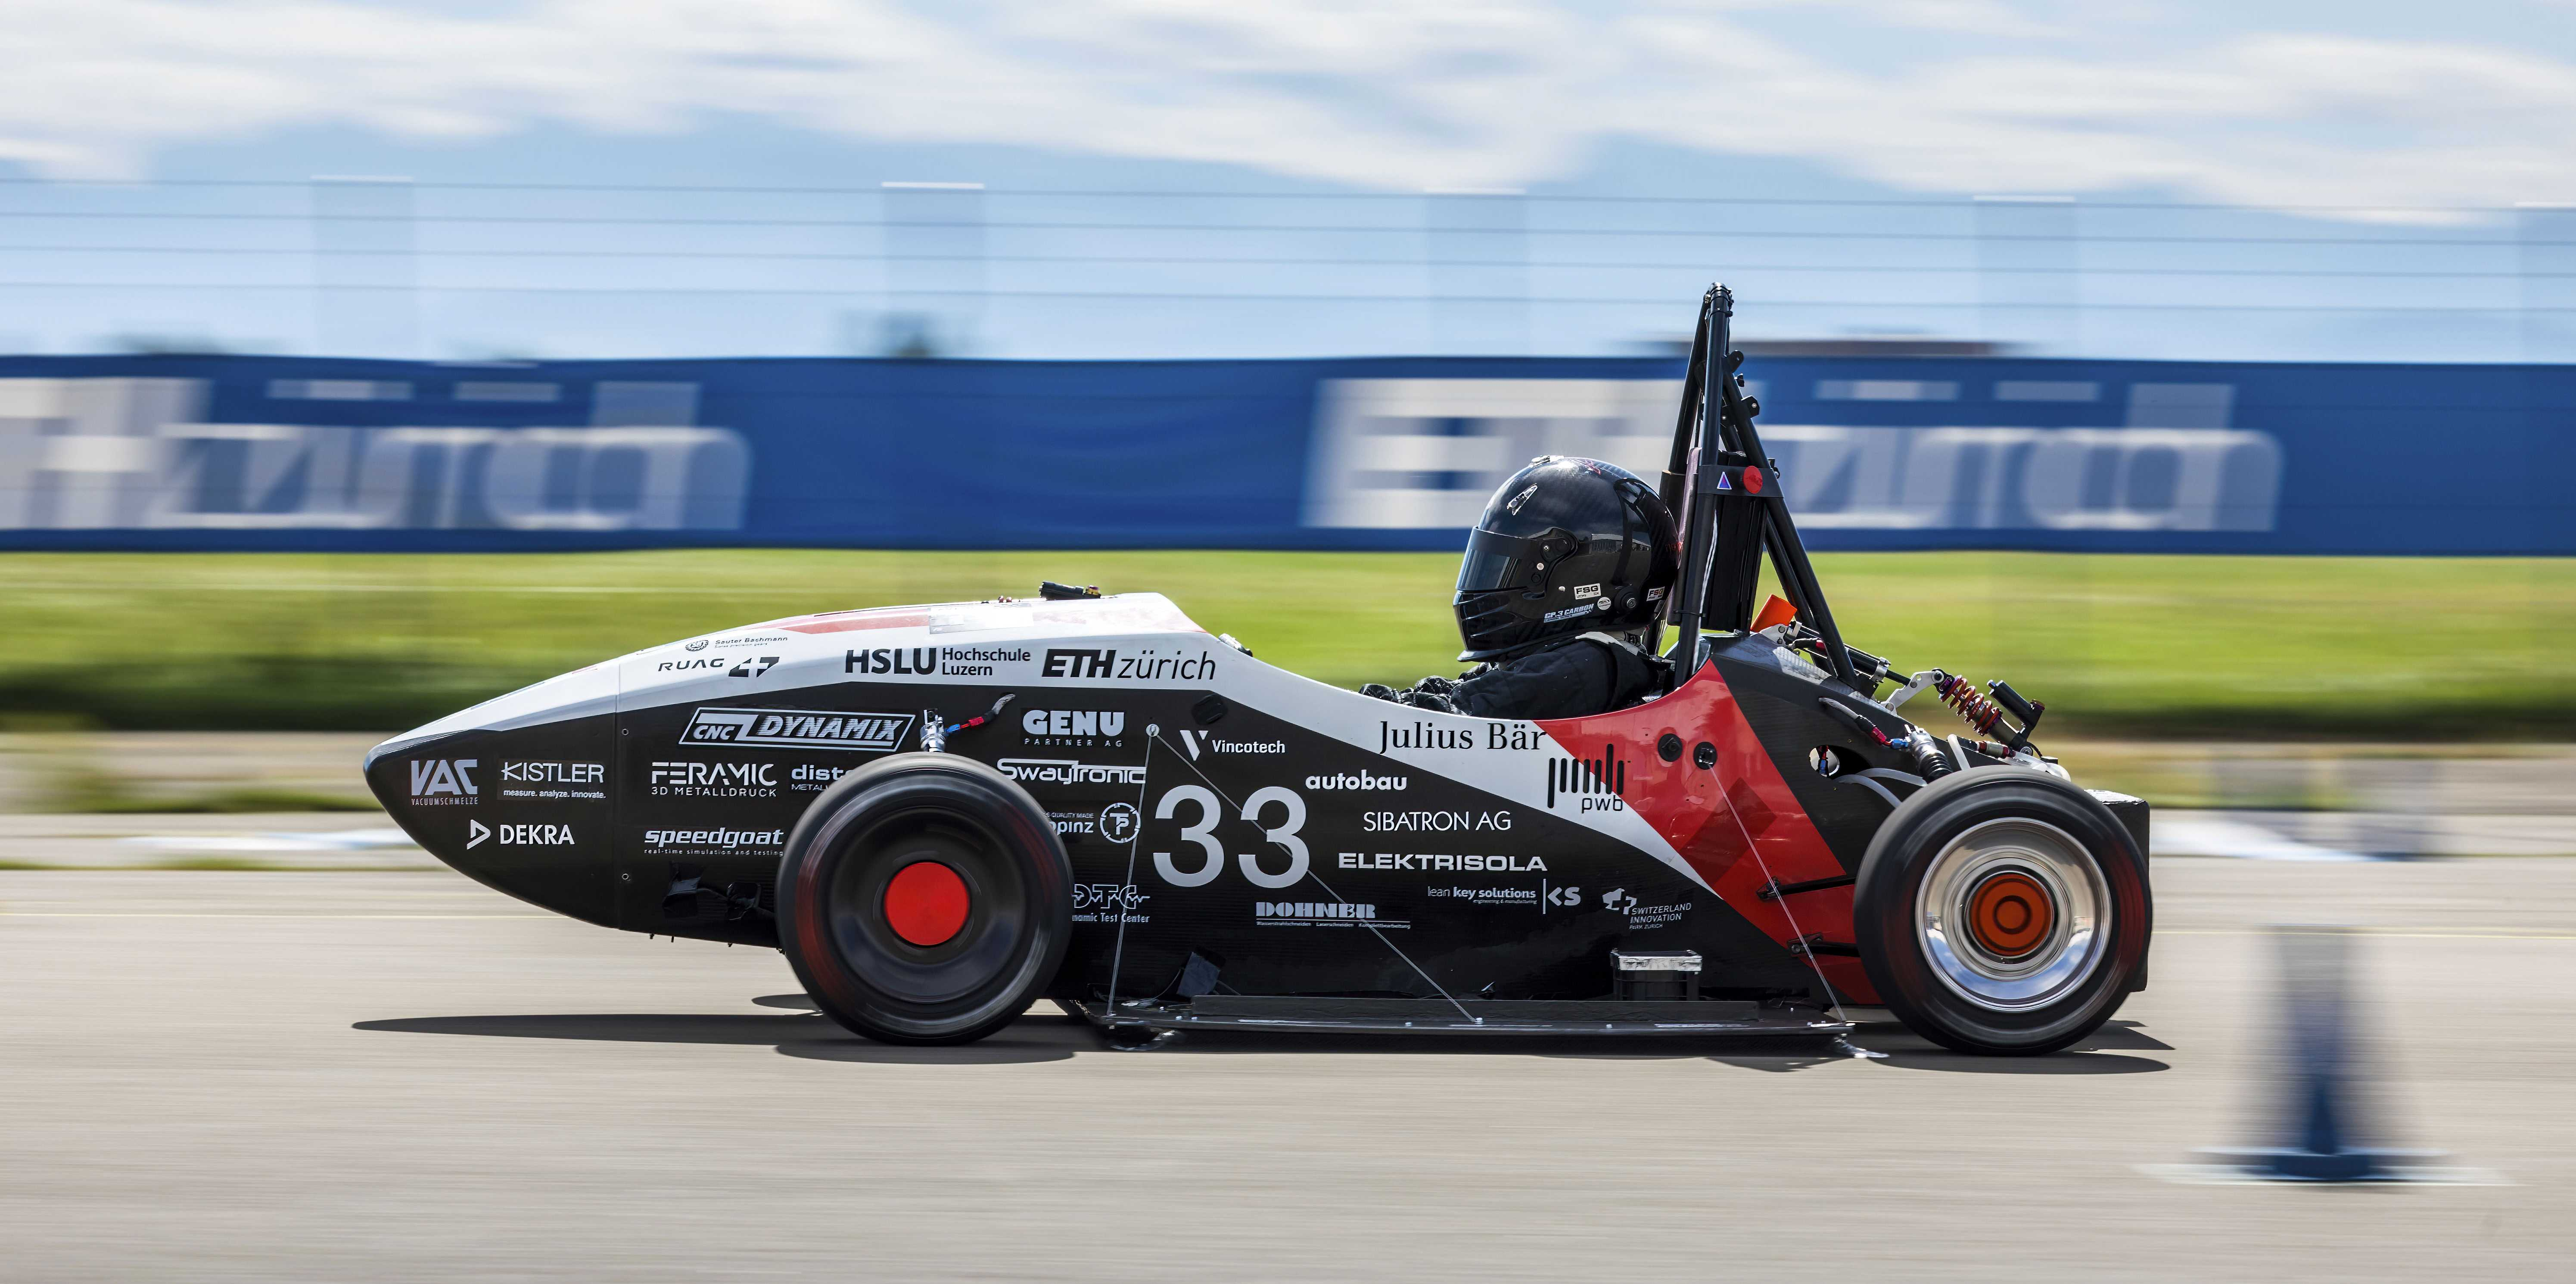
\includegraphics[width=0.85\linewidth]{Bilder/mythen.jpg}\\
\footnotesize Der Elektrorennwagen \emph{mythen} des Teams AMZ (ETH Zürich).
\end{center}

% Rekordwert verifiziert (September 2026, Quelle: ETH-Zürich-Medienmitteilung
% "From zero to one hundred in 0.956 seconds", 08.09.2023; weiterhin
% aktueller Guinness-Weltrekord, kein neuerer Rekord seither gefunden).
Das Studierendenteam AMZ (Akademischer Motorsportverein Zürich) der ETH
Zürich baut jedes Jahr einen eigenen Elektrorennwagen. Mit dem Fahrzeug
\emph{mythen} stellte das Team 2023 einen Guinness-Weltrekord auf: Der
Wagen beschleunigt von $\SI{0}{\kilo\meter\per\hour}$ auf
$\SI{100}{\kilo\meter\per\hour}$ in nur $\SI{0.956}{\second}$, über eine
Strecke von lediglich $\SI{12.3}{\meter}$, schneller als jedes andere
Elektroauto der Welt.

Wie schafft ein Elektroauto das? Ein Elektromotor liefert seine volle
Kraft bereits ab der ersten Umdrehung, während ein Benzinmotor erst
hochdrehen muss, bevor er seine grösste Kraft erreicht. Zusätzlich sitzt
bei \emph{mythen} an jedem der vier Räder ein eigener Motor, und das
Fahrzeug wiegt dank seiner Carbonbauweise nur einen Bruchteil eines
gewöhnlichen Autos. Viel Antriebskraft bei sehr wenig Gewicht: genau das
braucht es für eine derart extreme Beschleunigung.

Was fällt dir auf, wenn du diese Bewegung mit den gleichförmigen
Bewegungen vergleichst, die wir bisher untersucht haben? Bei
\emph{mythen} ist die Geschwindigkeit die ganze Zeit über
\textbf{\emph{unterschiedlich}}, sie nimmt laufend zu. Genau diese
Änderung der Geschwindigkeit über die Zeit nennen wir
\textbf{\emph{Beschleunigung}}, das Thema dieses Arbeitsblatts.

Manche Darstellungen einer solchen Bewegung sehen im $s$-$t$-Diagramm
so aus:

\begin{center}
\begin{tikzpicture}[scale=0.85]
  \draw[gray!20] (0,0) grid[xstep=1,ystep=1] (6,8);
  \draw[->] (-0.3,0) -- (6.5,0) node[right] {\scriptsize $t$};
  \draw[->] (0,-0.3) -- (0,8.5) node[above] {\scriptsize $s$};
  \foreach \x in {1,2,3,4,5,6} \draw (\x,0.08) -- (\x,-0.08) node[below] {\scriptsize \x};
  \foreach \y in {1,3.5,8} \draw (0.08,\y) -- (-0.08,\y) node[left] {\scriptsize \y};
  \draw[thick,titleblue] (0,0) -- (2,1) -- (4,3.5) -- (6,8);
  \filldraw[black] (0,0) circle (1.6pt);
  \filldraw[black] (2,1) circle (1.6pt);
  \filldraw[black] (4,3.5) circle (1.6pt);
  \filldraw[black] (6,8) circle (1.6pt);
\end{tikzpicture}
\end{center}

Ist das eine korrekte Darstellung der Wirklichkeit? Das untersuchst du
gleich in der folgenden Übung.
\end{beispielbox}

\begin{questions}
\begin{taskbox}[Übung: v-t-Diagramm zum Einstiegsbeispiel]
\question[4] Zeichne zum $s$-$t$-Diagramm aus dem Einstieg oben das
dazugehörige $v$-$t$-Diagramm für die drei Streckenabschnitte, und
beurteile anschliessend, ob diese Bewegung physikalisch sinnvoll ist.

\begin{center}
\begin{tikzpicture}[scale=1.3]
  \draw[gray!20] (0,0) grid[xstep=1,ystep=0.5] (6,3);
  \draw[->] (-0.3,0) -- (6.5,0) node[right] {\scriptsize $t$};
  \draw[->] (0,-0.3) -- (0,3.3) node[above] {\scriptsize $v$};
  \foreach \x in {1,2,3,4,5,6} \draw (\x,0.08) -- (\x,-0.08) node[below] {\scriptsize \x};
  \foreach \y in {0.5,1,1.5,2,2.5} \draw (0.08,\y) -- (-0.08,\y) node[left] {\scriptsize \y};
\end{tikzpicture}
\end{center}

\Antwortraum{4}
\begin{solution}
Die drei Streckenabschnitte im $s$-$t$-Diagramm haben je eine konstante,
aber unterschiedliche Steigung, also ist $v$ in jedem Abschnitt konstant:
\[
  v_1=\frac{1-0}{2-0}=0.5, \qquad
  v_2=\frac{3.5-1}{4-2}=1.25, \qquad
  v_3=\frac{8-3.5}{6-4}=2.25.
\]
Das $v$-$t$-Diagramm besteht deshalb aus drei waagrechten Linien:

\begin{center}
\begin{tikzpicture}[scale=1.3]
  \draw[gray!20] (0,0) grid[xstep=1,ystep=0.5] (6,3);
  \draw[->] (-0.3,0) -- (6.5,0) node[right] {\scriptsize $t$};
  \draw[->] (0,-0.3) -- (0,3.3) node[above] {\scriptsize $v$};
  \foreach \x in {1,2,3,4,5,6} \draw (\x,0.08) -- (\x,-0.08) node[below] {\scriptsize \x};
  \foreach \y in {0.5,1,1.5,2,2.5} \draw (0.08,\y) -- (-0.08,\y) node[left] {\scriptsize \y};
  \draw[thick,accentorange] (0,0.5) -- (2,0.5);
  \draw[dashed,gray] (2,0.5) -- (2,1.25);
  \draw[thick,accentorange] (2,1.25) -- (4,1.25);
  \draw[dashed,gray] (4,1.25) -- (4,2.25);
  \draw[thick,accentorange] (4,2.25) -- (6,2.25);
\end{tikzpicture}
\end{center}

An den beiden Knicken (bei $t=2$ und $t=4$) springt die Geschwindigkeit
sprunghaft von einem Wert zum nächsten, in null Zeit. Das entspricht
einer unendlich grossen Beschleunigung für einen einzelnen Moment
($a=\Delta v/\Delta t$ mit $\Delta t \to 0$) und ist physikalisch
\textbf{\emph{nicht sinnvoll}}: Kein reales Objekt kann seine
Geschwindigkeit augenblicklich ändern.
\end{solution}
\end{taskbox}
\end{questions}

\begin{questions}
\setcounter{question}{1}
\begin{taskbox}[Übung: Realistisches Beschleunigungsdiagramm]
\question[3] Du hast in der Übung oben erkannt, dass die Knicke im
$s$-$t$-Diagramm aus dem Einstieg eine sprunghafte, physikalisch nicht
sinnvolle Geschwindigkeitsänderung bedeuten. Skizziere stattdessen ein
$s$-$t$-Diagramm für dieselbe Bewegung (Start bei $s=0$, ungefähr
dieselbe Endposition), bei dem die Geschwindigkeit
\textbf{\emph{kontinuierlich}} zunimmt.

\begin{center}
\begin{tikzpicture}[scale=0.85]
  \draw[gray!20] (0,0) grid[xstep=1,ystep=1] (6,8);
  \draw[->] (-0.3,0) -- (6.5,0) node[right] {\scriptsize $t$};
  \draw[->] (0,-0.3) -- (0,8.5) node[above] {\scriptsize $s$};
\end{tikzpicture}
\end{center}

\begin{solution}
\begin{center}
\begin{tikzpicture}[scale=0.85]
  \draw[gray!20] (0,0) grid[xstep=1,ystep=1] (6,8);
  \draw[->] (-0.3,0) -- (6.5,0) node[right] {\scriptsize $t$};
  \draw[->] (0,-0.3) -- (0,8.5) node[above] {\scriptsize $s$};
  \draw[thick,accentorange,domain=0:6,samples=60,smooth] plot (\x,{(2/9)*\x*\x});
  \filldraw[black] (0,0) circle (1.6pt);
  \filldraw[black] (6,8) circle (1.6pt);
\end{tikzpicture}
\end{center}
Bei kontinuierlicher Beschleunigung ist das $s$-$t$-Diagramm eine glatte
Kurve, zum Beispiel eine Parabel bei konstanter Beschleunigung, nicht
eine Folge von Geradenstücken mit Knicken. Ein Knick würde bedeuten,
dass sich die Geschwindigkeit in null Zeit ändert, und das ist
physikalisch nicht möglich.
\end{solution}
\end{taskbox}
\end{questions}

% =============================================================================
% Theorie: fachliche Grundlage für die Aufgaben, in eigene Boxen unterteilt
% (je Unterthema eine theoriebox), Reihenfolge = Lernziele-Reihenfolge oben.
% =============================================================================
\begin{theoriebox}[Beschleunigung: Änderungsrate der Geschwindigkeit]
Die \textbf{\emph{Beschleunigung}} $a$ eines Objekts beschreibt, wie
schnell sich seine \textbf{\emph{Geschwindigkeit}} $v$ mit der Zeit
ändert. Sie beschreibt nicht, wie schnell sich das Objekt selbst bewegt.

Ein Objekt kann sehr schnell unterwegs sein (grosses $v$) und dabei
trotzdem überhaupt nicht beschleunigen, wenn seine Geschwindigkeit
konstant bleibt ($a=0$). Umgekehrt kann ein Objekt, das sich erst
langsam bewegt, stark beschleunigen, wenn sich seine Geschwindigkeit
sehr schnell ändert.

\begin{formelbox}[Formel: Beschleunigung]
Allgemein berechnet sich die Beschleunigung als Änderungsrate der
Geschwindigkeit:
\[
  a = \frac{\Delta v}{\Delta t}, \qquad
  \text{Einheit von } a\colon\ \si{\meter\per\second\squared}.
\]
Wie die Geschwindigkeit $v$ ist auch die Beschleunigung $a$ eine
\textbf{\emph{gerichtete Grösse}} (mehr dazu weiter unten).
\end{formelbox}

\begin{center}
\begin{tikzpicture}[scale=0.9]
  \draw[->] (-0.3,0) -- (6.2,0) node[right] {\scriptsize $t$};
  \draw[->] (0,-0.3) -- (0,4.3) node[above] {\scriptsize $v$ in $\si{\kilo\meter\per\hour}$};
  \draw (0.1,3.69) -- (-0.1,3.69) node[left] {\scriptsize 120};
  \draw[dashed,gray] (0,3.69) -- (5.7,3.69);
  \draw[thick,titleblue] (0,3.69) -- (5.7,3.69) node[right] {\scriptsize Zug: konstant ($a=0$)};
  \draw (0.1,0.31) -- (-0.1,0.31) node[left] {\scriptsize 10};
  \draw[thick,accentorange] (0,0) -- (5.7,0.31) node[right] {\scriptsize Fahrrad: $0\to\SI{10}{\kilo\meter\per\hour}$ ($a\neq0$)};
\end{tikzpicture}
\end{center}

\textbf{Wichtig:} \emph{Schnell sein} (grosses $v$) und \emph{stark
beschleunigen} (grosses $a$) sind zwei ganz unterschiedliche Dinge, die
häufig verwechselt werden. Der Zug oben ist die ganze Zeit viel
schneller als das Fahrrad und liegt deshalb massstabsgetreu weit über
ihm, beschleunigt aber gar nicht: Seine Linie ist waagrecht, während die
viel tiefer liegende Linie des Fahrrads ansteigt.
\end{theoriebox}

\begin{questions}
\setcounter{question}{2}
\begin{taskbox}[Übung: Beschleunigung aus dem v-t-Diagramm berechnen]
\question[3] Genau wie sich im $s$-$t$-Diagramm die Geschwindigkeit als
Steigung der Geraden berechnen lässt, lässt sich im $v$-$t$-Diagramm die
Beschleunigung als deren Steigung berechnen. Bestimme mit einem
Steigungsdreieck die Beschleunigung $a$ der folgenden Bewegung.

\begin{center}
\begin{tikzpicture}[scale=0.75]
  \draw[gray!20] (0,0) grid[xstep=1,ystep=1] (6,10);
  \draw[->] (-0.3,0) -- (6.5,0) node[right] {\scriptsize $t$ in s};
  \draw[->] (0,-0.3) -- (0,10.5) node[above] {\scriptsize $v$ in $\si{\meter\per\second}$};
  \foreach \x in {1,2,3,4,5,6} \draw (\x,0.1) -- (\x,-0.1) node[below] {\scriptsize \x};
  \foreach \y in {2,4,6,8,10} \draw (0.1,\y) -- (-0.1,\y) node[left] {\scriptsize \y};
  \draw[thick,titleblue] (1,2) -- (5,10);
  \filldraw[black] (1,2) circle (1.6pt);
  \filldraw[black] (5,10) circle (1.6pt);
\end{tikzpicture}
\end{center}

\Antwortraum{3}
\begin{solution}
Steigungsdreieck: $4$ Kästchen nach rechts ($\Delta t=\SI{4}{\second}$),
$8$ Kästchen nach oben ($\Delta v=\SI{8}{\meter\per\second}$).
\[
  a = \frac{\Delta v}{\Delta t} = \frac{8}{4}\,\si{\meter\per\second\squared} = \SI{2}{\meter\per\second\squared}.
\]
\end{solution}
\end{taskbox}
\end{questions}

% Durchschnitts-/Momentanbeschleunigung (Sekante/Tangente, LZ2/LZ3) steht
% bewusst erst am Ende des Arbeitsblatts, siehe dortige theoriebox.

% Weg-Zeit-Formel s=1/2 a t^2: eigentlich Stoff der Bewegungsgleichungen-
% Einheit (siehe lernziele.md dieses Ordners, "Nicht Teil dieser Einheit"),
% hier auf ausdrücklichen Wunsch trotzdem eingeführt (Spezialfall v0=0).
% Statt sie direkt als theoriebox hinzustellen, leiten die SuS sie zuerst
% selbst her: Fläche im v-t-Diagramm (Dreieck) -> s=1/2*v*t -> v=a*t
% einsetzen -> s=1/2*a*t^2. Die vollständige/allgemeine Herleitung (inkl.
% v0!=0, dritte Bewegungsgleichung) bleibt in mechanik/bewegungsgleichungen/,
% hier nur dieser eine Spezialfall.
\begin{questions}
\setcounter{question}{3}
\begin{taskbox}[Herleitung: Weg aus der Fläche im v-t-Diagramm]
\question[4] Ein Objekt startet aus der Ruhe ($v_0=0$) und beschleunigt
gleichmässig (konstantes $a$). Nach der Zeit $t$ hat es die Geschwindigkeit
$v$ erreicht. Das $v$-$t$-Diagramm dieser Bewegung sieht so aus:

\begin{center}
\begin{tikzpicture}[scale=0.9]
  \draw[->] (-0.3,0) -- (5.5,0) node[right] {\scriptsize $t$};
  \draw[->] (0,-0.3) -- (0,4.3) node[above] {\scriptsize $v$};
  \filldraw[lightblue] (0,0) -- (4,3.2) -- (4,0) -- cycle;
  \draw[thick,titleblue] (0,0) -- (4,3.2);
  \draw[dashed,gray] (4,0) -- (4,3.2);
  \draw (4,0.08) -- (4,-0.08) node[below] {\scriptsize $t$};
  \draw (0.08,3.2) -- (-0.08,3.2) node[left] {\scriptsize $v$};
\end{tikzpicture}
\end{center}

\begin{parts}
  \part[2] Du kennst bereits aus dem $v$-$t$-Diagramm: Die Fläche zwischen
  der Kurve und der $t$-Achse entspricht der zurückgelegten Strecke $s$.
  Diese Fläche ist ein Dreieck. Stelle eine Formel für $s$ in Abhängigkeit
  von $v$ und $t$ auf.
  \Antwortraum{2}
  \begin{solution}
  Fläche eines Dreiecks $=\tfrac12\cdot\text{Grundseite}\cdot\text{Höhe}
  =\tfrac12\cdot t\cdot v$. Also:
  \[
    s = \frac12\,v\,t.
  \]
  \end{solution}

  \part[2] Aus der allgemeinen Beschleunigungsformel von ganz oben folgt
  für diese Bewegung aus dem Stand $v=a\cdot t$. Setze das in deine
  Formel für $s$ ein, und vereinfache so weit wie möglich.
  \Antwortraum{2}
  \begin{solution}
  Einsetzen von $v=a\cdot t$ in $s=\tfrac12\,v\,t$:
  \[
    s = \frac12\,(a\,t)\,t
  \]
  Zusammenfassen:
  \[
    s = \frac12\,a\,t^2.
  \]
  Das ist genau die Formel \glqq Weg aus dem Stand\grqq{}, die im nächsten
  Abschnitt festgehalten wird.
  \end{solution}
\end{parts}
\end{taskbox}
\end{questions}

\begin{theoriebox}[Weg bei gleichmässig beschleunigter Bewegung]
Wie du in der Übung oben hergeleitet hast: Startet ein Objekt aus der
Ruhe ($v_0=0$) und bewegt es sich anschliessend
\textbf{\emph{gleichmässig beschleunigt}}, also mit konstantem $a$, lässt
sich die zurückgelegte Strecke $s$ direkt aus $a$ und $t$ berechnen:

\begin{formelbox}[Formel: Weg aus dem Stand]
\[
  s = \frac{1}{2}\,a\,t^2, \qquad \text{Einheit von } s\colon\ \si{\meter}.
\]
\end{formelbox}

Die Beschleunigung $a$ bestimmt dabei, wie steil die Kurve im
$s$-$t$-Diagramm nach oben wächst: Je grösser $a$, desto schneller nimmt
$s$ mit der Zeit zu.

\begin{center}
\begin{tikzpicture}[scale=0.9]
  \draw[->] (-0.3,0) -- (5.7,0) node[right] {\scriptsize $t$};
  \draw[->] (0,-0.3) -- (0,5) node[above] {\scriptsize $s$};
  \draw[thick,accentorange,domain=0:5,samples=60,smooth] plot (\x,{0.18*\x*\x});
  \node[accentorange,right] at (5,4.5) {\scriptsize grosses $a$};
  \draw[thick,titleblue,domain=0:5,samples=60,smooth] plot (\x,{0.06*\x*\x});
  \node[titleblue,right] at (5,1.5) {\scriptsize kleines $a$};
\end{tikzpicture}
\end{center}

Beide Kurven sind \textbf{\emph{Parabeln}}: $s(t)=\tfrac12 a t^2$ ist eine
\textbf{\emph{quadratische Funktion}} von $t$, deshalb die charakteristische
gekrümmte Form, unabhängig davon, wie gross $a$ ist.
\end{theoriebox}

% Herleitung s=v^2/(2a) ("3. Bewegungsgesetz"): wie die Weg-Zeit-Formel
% oben eigentlich Stoff von mechanik/bewegungsgleichungen/ (siehe
% lernziele.md, "Nicht Teil dieser Einheit"), hier auf ausdrücklichen
% Wunsch trotzdem ergänzt, direkt im Anschluss an die Formel, aus der sie
% hergeleitet wird.
\begin{questions}
\setcounter{question}{4}
\begin{taskbox}[Herleitung: Weg in Abhängigkeit von v und a]
\question[3] Aus der Formel für die Beschleunigung von ganz oben folgt für
eine Bewegung aus dem Stand ($v_0=0$): $a=\dfrac{v}{t}$, also
$t=\dfrac{v}{a}$. Setze diesen Ausdruck für $t$ in die Formel
$s=\tfrac12 a t^2$ von oben ein, und vereinfache so weit wie möglich, bis
du eine Formel für $s$ erhältst, die nur noch $v$ und $a$ enthält (aber
kein $t$ mehr).
\Antwortraum{3}
\begin{solution}
Einsetzen von $t=\dfrac{v}{a}$ in $s=\tfrac12 a t^2$:
\[
  s = \frac12\,a\left(\frac{v}{a}\right)^2
\]
Klammer auflösen (Bruch quadrieren):
\[
  s = \frac12\,a\cdot\frac{v^2}{a^2}
\]
Ein $a$ kürzen:
\[
  s = \frac{v^2}{2a}.
\]
\end{solution}
\end{taskbox}
\end{questions}

\begin{theoriebox}[Zwei Grundtypen der Bewegung im Vergleich]
Ob eine Bewegung im $s$-$t$-, $v$-$t$- und $a$-$t$-Diagramm als Gerade,
waagrechte Linie oder Kurve erscheint, hängt davon ab, \emph{was} konstant
bleibt: die Geschwindigkeit oder die Beschleunigung. Die beiden
wichtigsten Grundtypen im Vergleich:

\textbf{\emph{Gleichförmige Bewegung}} ($v=\text{konst.}$, also $a=0$):

\begin{center}
\begin{minipage}{0.30\linewidth}\centering
\begin{tikzpicture}[scale=0.62]
  \draw[->] (-0.3,0) -- (5,0) node[right] {\scriptsize $t$};
  \draw[->] (0,-0.3) -- (0,4.3) node[above] {\scriptsize $s$};
  \draw[thick,titleblue] (0,0) -- (4.5,3.6);
  \node[right] at (4.5,3.6) {\tiny $s=v\cdot t$};
\end{tikzpicture}\\[-0.2em]
{\scriptsize $s$-$t$: Gerade (Steigung $=v$)}
\end{minipage}\hfill
\begin{minipage}{0.30\linewidth}\centering
\begin{tikzpicture}[scale=0.62]
  \draw[->] (-0.3,0) -- (5,0) node[right] {\scriptsize $t$};
  \draw[->] (0,-0.3) -- (0,4.3) node[above] {\scriptsize $v$};
  \filldraw[lightblue] (0,0) rectangle (4.5,2.4);
  \draw[thick,titleblue] (0,2.4) -- (4.5,2.4);
  \draw[dashed,gray] (4.5,0) -- (4.5,2.4);
  \node at (2.25,2.75) {\tiny $v=\text{konst.}$};
  \node[align=center] at (2.25,1.2) {\tiny Fläche\\$=v\cdot t=s$};
\end{tikzpicture}\\[-0.2em]
{\scriptsize $v$-$t$: waagrecht}
\end{minipage}\hfill
\begin{minipage}{0.30\linewidth}\centering
\begin{tikzpicture}[scale=0.62]
  \draw[->] (-0.3,0) -- (5,0) node[right] {\scriptsize $t$};
  \draw[->] (0,-0.3) -- (0,4.3) node[above] {\scriptsize $a$};
  \draw[thick,titleblue] (0,0) -- (4.5,0);
  \node at (2.25,0.5) {\tiny $a=0$};
\end{tikzpicture}\\[-0.2em]
{\scriptsize $a$-$t$: auf der $t$-Achse ($a=0$)}
\end{minipage}
\end{center}

\textbf{\emph{Gleichmässig beschleunigte Bewegung}} ($a=\text{konst.}\neq0$):

\begin{center}
\begin{minipage}{0.30\linewidth}\centering
\begin{tikzpicture}[scale=0.62]
  \draw[->] (-0.3,0) -- (5,0) node[right] {\scriptsize $t$};
  \draw[->] (0,-0.3) -- (0,4.3) node[above] {\scriptsize $s$};
  \draw[thick,accentorange,domain=0:4.5,samples=60,smooth] plot (\x,{0.18*\x*\x});
  \node[right] at (4.5,3.65) {\tiny $s=\tfrac12at^2$};
\end{tikzpicture}\\[-0.2em]
{\scriptsize $s$-$t$: Parabel (immer steiler)}
\end{minipage}\hfill
\begin{minipage}{0.30\linewidth}\centering
\begin{tikzpicture}[scale=0.62]
  \draw[->] (-0.3,0) -- (5,0) node[right] {\scriptsize $t$};
  \draw[->] (0,-0.3) -- (0,4.3) node[above] {\scriptsize $v$};
  \filldraw[lightblue] (0,0) -- (4.5,3.6) -- (4.5,0) -- cycle;
  \draw[thick,accentorange] (0,0) -- (4.5,3.6);
  \draw[dashed,gray] (4.5,0) -- (4.5,3.6);
  \node[right] at (4.5,3.6) {\tiny $v=a\cdot t$};
  \node[align=center] at (3.15,0.9) {\tiny Fläche\\$=\tfrac12at^2=s$};
\end{tikzpicture}\\[-0.2em]
{\scriptsize $v$-$t$: Gerade (Steigung $=a$)}
\end{minipage}\hfill
\begin{minipage}{0.30\linewidth}\centering
\begin{tikzpicture}[scale=0.62]
  \draw[->] (-0.3,0) -- (5,0) node[right] {\scriptsize $t$};
  \draw[->] (0,-0.3) -- (0,4.3) node[above] {\scriptsize $a$};
  \filldraw[lightblue] (0,0) rectangle (4.5,2.4);
  \draw[thick,accentorange] (0,2.4) -- (4.5,2.4);
  \draw[dashed,gray] (4.5,0) -- (4.5,2.4);
  \node at (2.25,2.75) {\tiny $a=\text{konst.}$};
  \node[align=center] at (2.25,1.2) {\tiny Fläche\\$=a\cdot t=\Delta v$};
\end{tikzpicture}\\[-0.2em]
{\scriptsize $a$-$t$: waagrecht, aber $\neq0$}
\end{minipage}
\end{center}

\textbf{Wichtig:} Bei konstanter Geschwindigkeit ist das $v$-$t$-Diagramm
waagrecht und das $a$-$t$-Diagramm liegt auf der Nulllinie. Bei
konstanter Beschleunigung ist stattdessen das $v$-$t$-Diagramm eine
Gerade und das $a$-$t$-Diagramm waagrecht, während das $s$-$t$-Diagramm
zu einer immer steiler werdenden Kurve wird. Das $a$-$t$-Diagramm allein
verrät also nicht, ob sich ein Objekt überhaupt bewegt. Dafür braucht
es das $v$-$t$- oder $s$-$t$-Diagramm.
\end{theoriebox}

\begin{questions}
\setcounter{question}{5}
\begin{taskbox}[Übung: Fläche unter der a-t-Kurve]
Du kennst bereits aus dem $v$-$t$-Diagramm: Die Fläche zwischen der Kurve
und der $t$-Achse entspricht der Ortsänderung $s$. Überlege mit demselben
Gedankengang, was die Fläche unter einer $a$-$t$-Kurve wohl bedeutet.

\question[2] Ein E-Trottinett startet aus dem Stand und beschleunigt
$\SI{4}{\second}$ lang konstant mit $a=\SI{1.5}{\meter\per\second\squared}$.

\begin{center}
\begin{tikzpicture}[scale=0.9]
  \draw[gray!20] (0,0) grid[xstep=1,ystep=1] (5,3);
  \draw[->] (-0.3,0) -- (5.5,0) node[right] {\scriptsize $t$ in s};
  \draw[->] (0,-0.3) -- (0,3.3) node[above] {\scriptsize $a$ in $\si{\meter\per\second\squared}$};
  \foreach \x in {1,2,3,4} \draw (\x,0.1) -- (\x,-0.1) node[below] {\scriptsize \x};
  \foreach \y in {1,1.5,2} \draw (0.1,\y) -- (-0.1,\y) node[left] {\scriptsize \y};
  \filldraw[lightblue] (0,0) rectangle (4,1.5);
  \draw[thick,titleblue] (0,1.5) -- (4,1.5);
  \draw[dashed,gray] (4,0) -- (4,1.5);
\end{tikzpicture}
\end{center}

\begin{parts}
  \part[1] Welche Einheit erhält man, wenn man $a$ (in
  $\si{\meter\per\second\squared}$) mit $t$ (in $\si{\second}$)
  multipliziert? Zu welcher physikalischen Grösse passt diese Einheit?
  \Antwortraum{1}
  \begin{solution}
  $\si{\meter\per\second\squared}\cdot\si{\second} = \si{\meter\per\second}$.
  Das ist die Einheit einer \emph{Geschwindigkeit}.
  \end{solution}

  \part[1] Berechne die Fläche unter der $a$-$t$-Kurve oben.
  \Antwortraum{1}
  \begin{solution}
  Fläche $= a\cdot\Delta t = \SI{1.5}{\meter\per\second\squared}\cdot\SI{4}{\second} = \SI{6}{\meter\per\second}$.
  \end{solution}
\end{parts}
\end{taskbox}
\end{questions}

\begin{questions}
\setcounter{question}{6}
\begin{taskbox}[Übung: Strecke bei gleichmässig beschleunigter Bewegung]
\question[6] Ein Auto startet bei einer Ampel aus dem Stand ($v_0=0$) und
beschleunigt $\SI{6}{\second}$ lang konstant mit
$a=\SI{1.5}{\meter\per\second\squared}$.

\begin{parts}
  \part[1] Bestimme die Geschwindigkeit $v_1$ am Ende der $\SI{6}{\second}$.
  \Antwortraum{1}
  \begin{solution}
  $v_1 = a\cdot t = \SI{1.5}{\meter\per\second\squared}\cdot\SI{6}{\second}
  = \SI{9}{\meter\per\second}$.
  \end{solution}

  \part[2] Zeichne das zugehörige $v$-$t$-Diagramm für diese
  $\SI{6}{\second}$.

  \begin{center}
  \begin{tikzpicture}[scale=0.7]
    \draw[gray!20] (0,0) grid[xstep=1,ystep=1] (7,10);
    \draw[->] (-0.3,0) -- (7.3,0) node[right] {\scriptsize $t$ in s};
    \draw[->] (0,-0.3) -- (0,10.3) node[above] {\scriptsize $v$ in $\si{\meter\per\second}$};
    \foreach \x in {1,2,3,4,5,6} \draw (\x,0.1) -- (\x,-0.1) node[below] {\scriptsize \x};
    \foreach \y in {2,4,6,8} \draw (0.1,\y) -- (-0.1,\y) node[left] {\scriptsize \y};
  \end{tikzpicture}
  \end{center}
  \begin{solution}
  \begin{center}
  \begin{tikzpicture}[scale=0.7]
    \draw[gray!20] (0,0) grid[xstep=1,ystep=1] (7,10);
    \draw[->] (-0.3,0) -- (7.3,0) node[right] {\scriptsize $t$ in s};
    \draw[->] (0,-0.3) -- (0,10.3) node[above] {\scriptsize $v$ in $\si{\meter\per\second}$};
    \foreach \x in {1,2,3,4,5,6} \draw (\x,0.1) -- (\x,-0.1) node[below] {\scriptsize \x};
    \foreach \y in {2,4,6,8} \draw (0.1,\y) -- (-0.1,\y) node[left] {\scriptsize \y};
    \draw (0.1,9) -- (-0.1,9) node[left] {\scriptsize 9};
    \filldraw[lightblue] (0,0) -- (6,9) -- (6,0) -- cycle;
    \draw[thick,titleblue] (0,0) -- (6,9);
    \draw[dashed,gray] (6,0) -- (6,9);
  \end{tikzpicture}
  \end{center}
  \end{solution}

  \part[3] Bestimme mithilfe der Fläche in deinem $v$-$t$-Diagramm die in
  diesen $\SI{6}{\second}$ zurückgelegte Strecke $s$.
  \Antwortraum{3}
  \begin{solution}
  Die Fläche ist ein Dreieck:
  \[
    s = \frac12\cdot t\cdot v_1 = \frac12\cdot\SI{6}{\second}\cdot\SI{9}{\meter\per\second} = \SI{27}{\meter}.
  \]
  \textbf{Probe} (Formel \glqq Weg aus dem Stand\grqq{}):
  $s=\tfrac12 a t^2 = \tfrac12\cdot\SI{1.5}{\meter\per\second\squared}\cdot(\SI{6}{\second})^2 = \SI{27}{\meter}$.
  Das stimmt überein.
  \end{solution}
\end{parts}
\end{taskbox}
\end{questions}

\begin{theoriebox}[Beschleunigung als Vektor]
Die Beschleunigung $a$ ist als Änderungsrate der Geschwindigkeit $v$
definiert. Weil $v$ selbst eine gerichtete Grösse ist, ein Vektor mit
Richtung und Wert, ist auch $a$ ein \textbf{\emph{Vektor}}: Sie hat, genau
wie $v$, sowohl eine \textbf{\emph{Richtung}} als auch einen
\textbf{\emph{Wert}} (Einheit: $\si{\meter\per\second\squared}$).

\begin{center}
\begin{tikzpicture}[scale=0.85,>=Latex]
  \draw[->,thick,titleblue] (-2.5,0) -- (3,0) node[right] {\scriptsize positive Richtung};
  \filldraw[black] (-1.5,0) circle (2pt);
  \draw[->,thick,red] (-1.5,0.6) -- (1.3,0.6) node[midway,above] {\scriptsize $v$};
  \draw[->,thick,green!55!black] (-1.5,-0.6) -- (-0.2,-0.6) node[midway,below] {\scriptsize $a$};
\end{tikzpicture}\\[0.2em]
{\scriptsize Ein Objekt zu einem bestimmten Zeitpunkt: Der rote Pfeil ist
der Geschwindigkeitsvektor $v$, der grüne Pfeil der
Beschleunigungsvektor $a$. Beide sind eigenständige Vektoren mit
eigener Richtung und eigenem Wert (Pfeillänge), die nicht
übereinstimmen müssen.}
\end{center}

Siehst du $v$ oder $a$ als Pfeil in einem Bild (etwa in der folgenden
Übung oder im $v$-$t$-Diagramm), zeigt dieser Pfeil immer nur die
Situation zu einem \textbf{\emph{einzigen Zeitpunkt}}, wie eine
Momentaufnahme. Wird der $v$-Pfeil zu einem späteren Zeitpunkt länger
oder kürzer, oder dreht er sogar die Richtung, dann ist genau das die
Beschleunigung: $a$ beschreibt \emph{diese Änderung} des $v$-Pfeils.
Umgekehrt gilt ebenso: $v$ kann sich nur ändern, wenn eine Beschleunigung
vorliegt. Ohne Beschleunigung ($a=0$) bleibt der $v$-Pfeil, also die
Geschwindigkeit, für immer exakt gleich; die Beschleunigung ist der
Grund für jede Änderung von $v$.

Wie die Geschwindigkeit trägt also auch die Beschleunigung ein
\textbf{\emph{Vorzeichen}}, das ihre Richtung relativ zu einem gewählten
Koordinatensystem angibt, unabhängig davon, ob das Objekt schneller
oder langsamer wird.

\textbf{Wichtig:} Eine \emph{negative} Beschleunigung bedeutet
\textbf{nicht} automatisch \textbf{\emph{Verzögerung}} (langsamer
werden), und eine \emph{positive} Beschleunigung bedeutet nicht
automatisch schneller werden. Entscheidend ist, ob $v$ und $a$ dasselbe
oder unterschiedliches Vorzeichen haben:
\begin{itemize}[leftmargin=1.2cm,itemsep=0.25em]
  \item $v$ und $a$ haben \textbf{\emph{dasselbe}} Vorzeichen
  $\Rightarrow$ das Objekt wird schneller (der Betrag von $v$ nimmt zu).
  \item $v$ und $a$ haben \textbf{\emph{unterschiedliches}} Vorzeichen
  $\Rightarrow$ das Objekt wird langsamer, es \textbf{\emph{verzögert}}
  (der Betrag von $v$ nimmt ab).
\end{itemize}

\begin{center}
\begin{minipage}{0.47\linewidth}\centering
\begin{tikzpicture}[scale=0.75,>=Latex]
  \draw[->,thick,titleblue] (-2.3,0) -- (2.6,0) node[right] {\scriptsize positive Richtung};
  \draw[->,thick,red] (-1.8,-0.6) -- (1.3,-0.6) node[midway,above] {\scriptsize $v$};
  \draw[->,thick,green!55!black] (-1.8,-1.3) -- (0.3,-1.3) node[midway,above] {\scriptsize $a$};
\end{tikzpicture}\\[-0.2em]
{\scriptsize dasselbe Vorzeichen $\Rightarrow$ schneller}
\end{minipage}\hfill
\begin{minipage}{0.47\linewidth}\centering
\begin{tikzpicture}[scale=0.75,>=Latex]
  \draw[->,thick,titleblue] (-2.3,0) -- (2.6,0) node[right] {\scriptsize positive Richtung};
  \draw[->,thick,red] (1.3,-0.6) -- (-1.8,-0.6) node[midway,above] {\scriptsize $v$};
  \draw[->,thick,green!55!black] (-1.8,-1.3) -- (0.8,-1.3) node[midway,above] {\scriptsize $a$};
\end{tikzpicture}\\[-0.2em]
{\scriptsize unterschiedliches Vorzeichen $\Rightarrow$ langsamer (verzögert)}
\end{minipage}
\end{center}
\end{theoriebox}

\begin{beispielbox}[Beispiel: Auto fährt nach links und wird langsamer]
Ein Auto bewegt sich nach links (das entspricht der \emph{negativen}
Richtung in unserem Koordinatensystem) und wird dabei immer langsamer.
Bei $t_1=\SI{0}{\second}$ beträgt seine Geschwindigkeit
$v_1=-\SI{12}{\meter\per\second}$, bei $t_2=\SI{4}{\second}$ nur noch
$v_2=-\SI{4}{\meter\per\second}$.

\begin{center}
\begin{tikzpicture}[scale=0.7]
  \draw[gray!20] (0,-13) grid[xstep=1,ystep=1] (5,1);
  \draw[->] (-0.3,0) -- (5.5,0) node[right] {\scriptsize $t$ in s};
  \draw[->] (0,-13.5) -- (0,1.5) node[above] {\scriptsize $v$ in $\si{\meter\per\second}$};
  \foreach \x in {4} \draw (\x,0.2) -- (\x,-0.2) node[below] {\scriptsize \x};
  \foreach \y in {-12,-8,-4,0} \draw (0.15,\y) -- (-0.15,\y) node[left] {\scriptsize \y};
  \draw[thick,titleblue] (0,-12) -- (4,-4);
  \filldraw[black] (0,-12) circle (1.6pt) node[below right] {\scriptsize $t_1$};
  \filldraw[black] (4,-4) circle (1.6pt) node[above left] {\scriptsize $t_2$};
\end{tikzpicture}
\end{center}

Werte einsetzen:
\[
  a = \frac{v_2 - v_1}{t_2 - t_1} = \frac{-\SI{4}{\meter\per\second} - (-\SI{12}{\meter\per\second})}{\SI{4}{\second}}.
\]
Zähler vereinfachen (\glqq minus minus\grqq{} wird \glqq plus\grqq{},
$-a-(-b)=-a+b$):
\[
  a = \frac{-\SI{4}{\meter\per\second} + \SI{12}{\meter\per\second}}{\SI{4}{\second}}
    = \frac{\SI{8}{\meter\per\second}}{\SI{4}{\second}}.
\]
Teilen:
\[
  a = +\SI{2}{\meter\per\second\squared}.
\]

Obwohl das Auto sich die ganze Zeit in die negative Richtung bewegt (und
dabei langsamer wird, also verzögert), ist seine Beschleunigung
\emph{positiv}. Der Grund: $v$ ist negativ und $a$ positiv, die beiden
Vorzeichen sind also unterschiedlich, und genau das bedeutet, dass das
Auto langsamer wird.
\end{beispielbox}

\begin{questions}
\setcounter{question}{7}
\begin{taskbox}[Übung: Simulation \glqq Der bewegte Mann\grqq{}]
\question[4] Öffne die PhET-Simulation \glqq Der bewegte Mann\grqq{} auf
LEIFIphysik:

\begin{center}
\small\url{https://www.leifiphysik.de/mechanik/lineare-bewegung-gleichungen/versuche/der-bewegte-mann-simulation-von-phet}
\end{center}

Wechsle dort zur \textbf{\emph{Diagrammansicht}} (Geschwindigkeits- und
Beschleunigungsdiagramm).

\begin{parts}
  \part[2] Stelle eine konstante, positive Beschleunigung ein, und starte
  den Mann aus der Ruhe ($v=0$). Beschreibe, wie sich der
  Geschwindigkeitsvektor (Pfeil) während der Bewegung verhält.
  \Antwortraum{2}
  \begin{solution}
  Der Geschwindigkeitsvektor zeigt die ganze Zeit in dieselbe Richtung wie
  der Beschleunigungsvektor und wird dabei \textbf{\emph{immer länger}}:
  Die Geschwindigkeit nimmt gleichmässig zu ($v=a\cdot t$), die Richtung
  bleibt dabei unverändert.
  \end{solution}

  \part[2] Stelle jetzt eine Beschleunigung ein, die der aktuellen
  Bewegungsrichtung des Mannes \textbf{\emph{entgegengerichtet}} ist. Was
  passiert mit dem Geschwindigkeitsvektor?
  \Antwortraum{2}
  \begin{solution}
  Der Geschwindigkeitsvektor wird mit der Zeit \textbf{\emph{kürzer}}: Der
  Mann verzögert. Wirkt die Beschleunigung lange genug weiter, wird die
  Geschwindigkeit null, und der Pfeil dreht anschliessend die Richtung: Der
  Mann bewegt sich rückwärts und wird dabei wieder schneller, jetzt in die
  neue Richtung. Das bestätigt die Regel von oben: Zeigen $v$ und $a$ in
  dieselbe Richtung, wird das Objekt schneller; zeigen sie in
  unterschiedliche Richtungen, wird es langsamer.
  \end{solution}
\end{parts}
\end{taskbox}
\end{questions}

\begin{questions}
\setcounter{question}{8}
\begin{taskbox}[Übung: Bewegung aus Geschwindigkeits- und Beschleunigungsvektor bestimmen]
Die folgenden Bilder zeigen jeweils ein Auto zum Zeitpunkt $t=0$. Die
blaue Achse markiert die positive Richtung des gewählten
Koordinatensystems, der rote Pfeil zeigt die Geschwindigkeit $v(0)$, und
der grüne Pfeil zeigt die Beschleunigung $a$, die während der ganzen
betrachteten Zeit konstant bleibt. Beschreibe für jedes Bild in Worten,
was mit dem Auto passiert, und skizziere anschliessend das $s$-$t$- und
das $v$-$t$-Diagramm für $t\geq0$. Weil die Achsen in den Bildern nicht
beziffert sind, genügt eine ungefähre Skizze: Vorzeichen, Steigung und
Krümmung müssen stimmen, exakte Werte sind nicht nötig.

\question[6]
\begin{center}
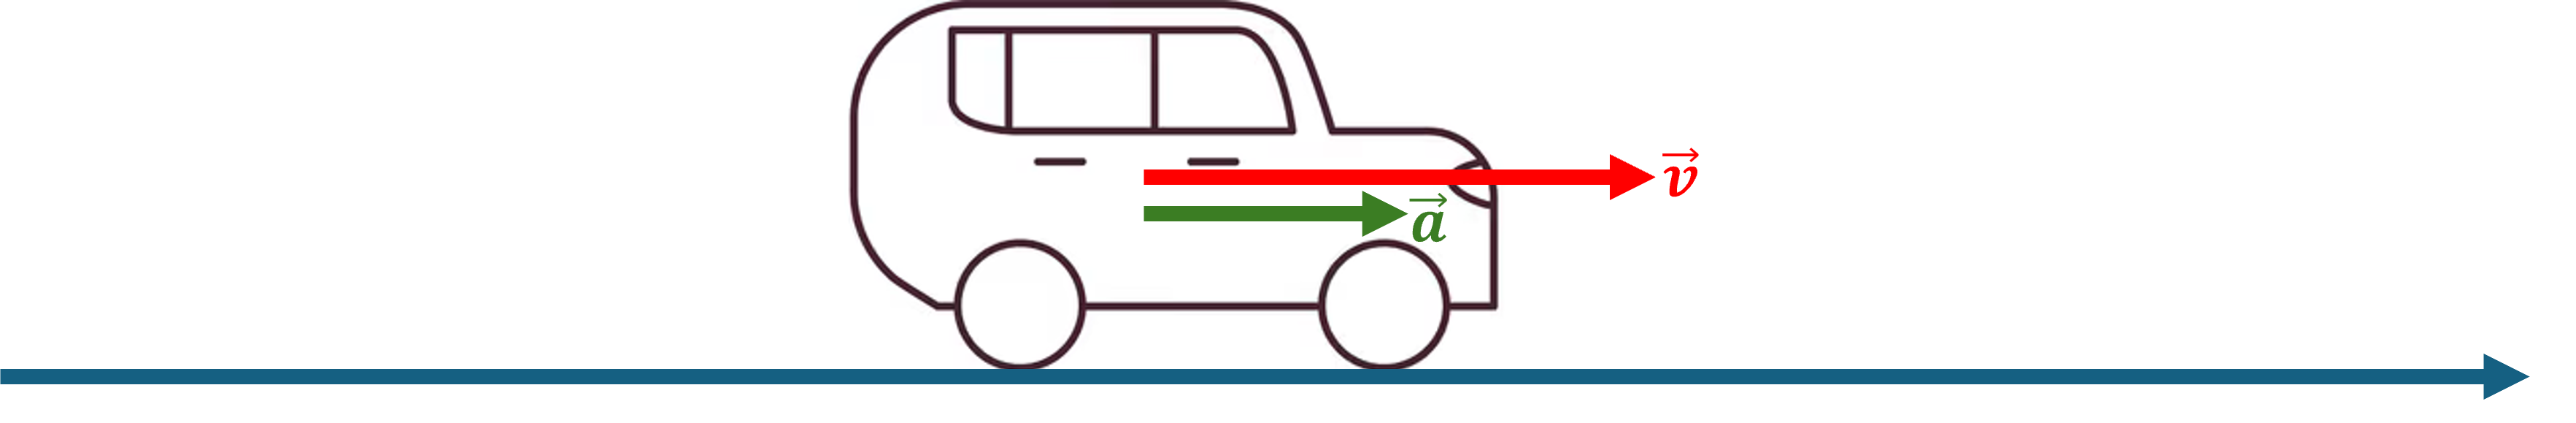
\includegraphics[width=0.9\linewidth]{Bilder/car_1.png}
\end{center}

\begin{parts}
  \part[2] Beschreibe in Worten, was mit dem Auto passiert.
  \Antwortraum{2}
  \begin{solution}
  Die Achse zeigt nach rechts, die positive Richtung ist also rechts.
  Sowohl $v$ als auch $a$ zeigen nach rechts, also gilt $v>0$ und $a>0$.
  Weil $v$ und $a$ dasselbe Vorzeichen haben, wird das Auto schneller,
  während es sich in die positive Richtung bewegt.
  \end{solution}

  \part[2] Skizziere das $s$-$t$-Diagramm.
  \begin{center}
  \begin{tikzpicture}[scale=0.6]
    \draw[->] (-0.3,0) -- (5.5,0) node[right] {\scriptsize $t$};
    \draw[->] (0,-3.5) -- (0,3.5) node[above] {\scriptsize $s$};
  \end{tikzpicture}
  \end{center}
  \begin{solution}
  \begin{center}
  \begin{tikzpicture}[scale=0.6]
    \draw[->] (-0.3,0) -- (5.5,0) node[right] {\scriptsize $t$};
    \draw[->] (0,-3.5) -- (0,3.5) node[above] {\scriptsize $s$};
    \draw[thick,titleblue,domain=0:4,samples=30,smooth] plot (\x,{0.5*\x+0.1*\x*\x});
  \end{tikzpicture}
  \end{center}
  Steigung bei $t=0$ positiv (weil $v>0$), und die Kurve wird immer
  steiler (weil $a>0$).
  \end{solution}

  \part[2] Skizziere das $v$-$t$-Diagramm.
  \begin{center}
  \begin{tikzpicture}[scale=0.6]
    \draw[->] (-0.3,0) -- (5.5,0) node[right] {\scriptsize $t$};
    \draw[->] (0,-3.5) -- (0,3.5) node[above] {\scriptsize $v$};
  \end{tikzpicture}
  \end{center}
  \begin{solution}
  \begin{center}
  \begin{tikzpicture}[scale=0.6]
    \draw[->] (-0.3,0) -- (5.5,0) node[right] {\scriptsize $t$};
    \draw[->] (0,-3.5) -- (0,3.5) node[above] {\scriptsize $v$};
    \draw[thick,titleblue] (0,0.8) -- (4,2.8);
  \end{tikzpicture}
  \end{center}
  Gerade mit positivem Achsenabschnitt (weil $v(0)>0$) und positiver
  Steigung (weil $a>0$).
  \end{solution}
\end{parts}

\needspace{10\baselineskip}
\question[6]
\begin{center}
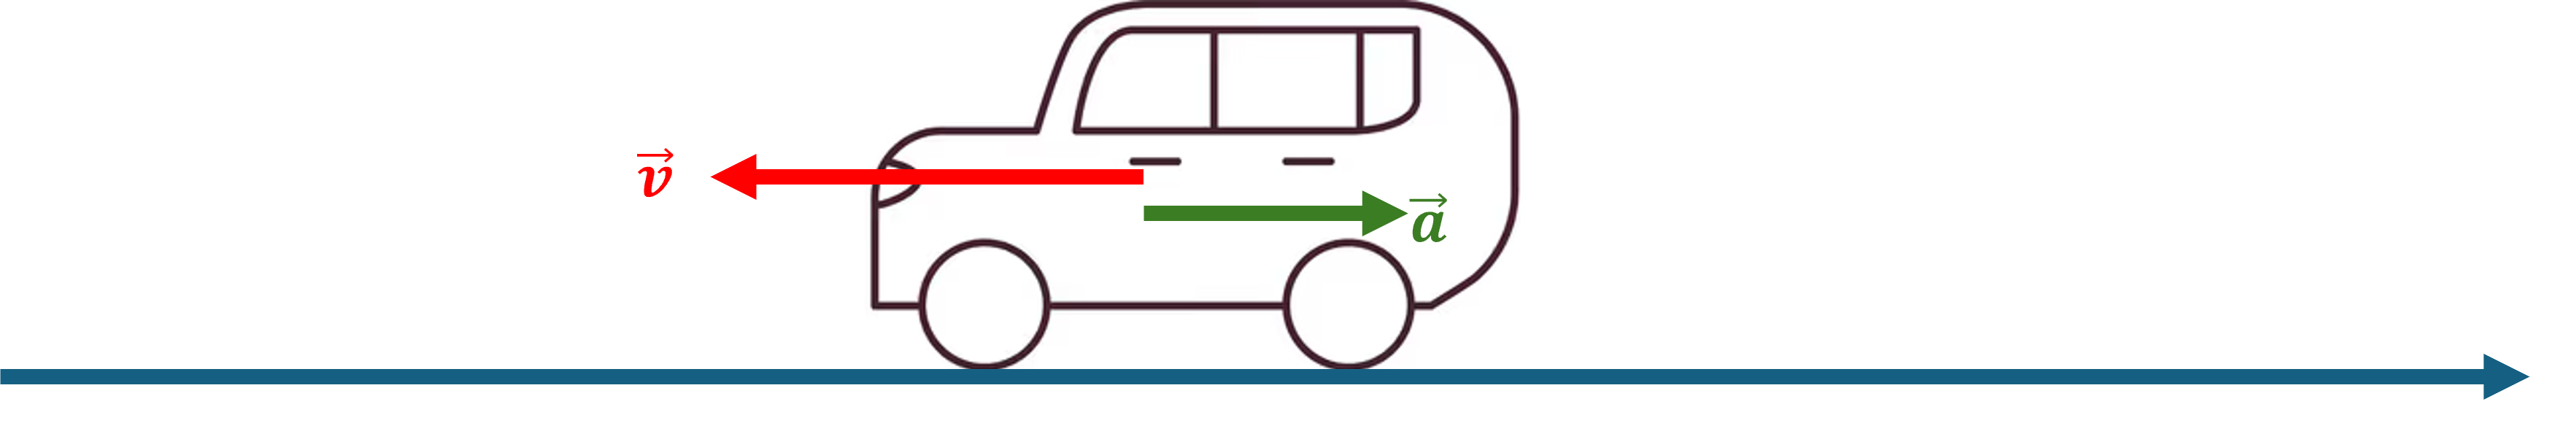
\includegraphics[width=0.9\linewidth]{Bilder/car_2.png}
\end{center}

\begin{parts}
  \part[2] Beschreibe in Worten, was mit dem Auto passiert.
  \Antwortraum{2}
  \begin{solution}
  Die Achse zeigt nach rechts, die positive Richtung ist also rechts.
  $v$ zeigt nach links, also gilt $v<0$. $a$ zeigt nach rechts, also gilt
  $a>0$. Weil $v$ und $a$ unterschiedliche Vorzeichen haben, wird das
  Auto langsamer, es verzögert, während es sich weiterhin in die
  negative Richtung bewegt.
  \end{solution}

  \part[2] Skizziere das $s$-$t$-Diagramm.
  \begin{center}
  \begin{tikzpicture}[scale=0.6]
    \draw[->] (-0.3,0) -- (5.5,0) node[right] {\scriptsize $t$};
    \draw[->] (0,-3.5) -- (0,3.5) node[above] {\scriptsize $s$};
  \end{tikzpicture}
  \end{center}
  \begin{solution}
  \begin{center}
  \begin{tikzpicture}[scale=0.6]
    \draw[->] (-0.3,0) -- (5.5,0) node[right] {\scriptsize $t$};
    \draw[->] (0,-3.5) -- (0,3.5) node[above] {\scriptsize $s$};
    \draw[thick,titleblue,domain=0:4,samples=30,smooth] plot (\x,{-0.7*\x+0.06*\x*\x});
  \end{tikzpicture}
  \end{center}
  Steigung bei $t=0$ negativ (weil $v<0$), die Kurve flacht aber
  zunehmend ab (weil $a>0$ der negativen Geschwindigkeit entgegenwirkt).
  \end{solution}

  \part[2] Skizziere das $v$-$t$-Diagramm.
  \begin{center}
  \begin{tikzpicture}[scale=0.6]
    \draw[->] (-0.3,0) -- (5.5,0) node[right] {\scriptsize $t$};
    \draw[->] (0,-3.5) -- (0,3.5) node[above] {\scriptsize $v$};
  \end{tikzpicture}
  \end{center}
  \begin{solution}
  \begin{center}
  \begin{tikzpicture}[scale=0.6]
    \draw[->] (-0.3,0) -- (5.5,0) node[right] {\scriptsize $t$};
    \draw[->] (0,-3.5) -- (0,3.5) node[above] {\scriptsize $v$};
    \draw[thick,titleblue] (0,-2.4) -- (4,-0.3);
  \end{tikzpicture}
  \end{center}
  Gerade mit negativem Achsenabschnitt (weil $v(0)<0$) und positiver
  Steigung (weil $a>0$), sie nähert sich der $t$-Achse an, ohne sie im
  gezeichneten Bereich zu erreichen.
  \end{solution}
\end{parts}

\needspace{10\baselineskip}
\question[6]
\begin{center}
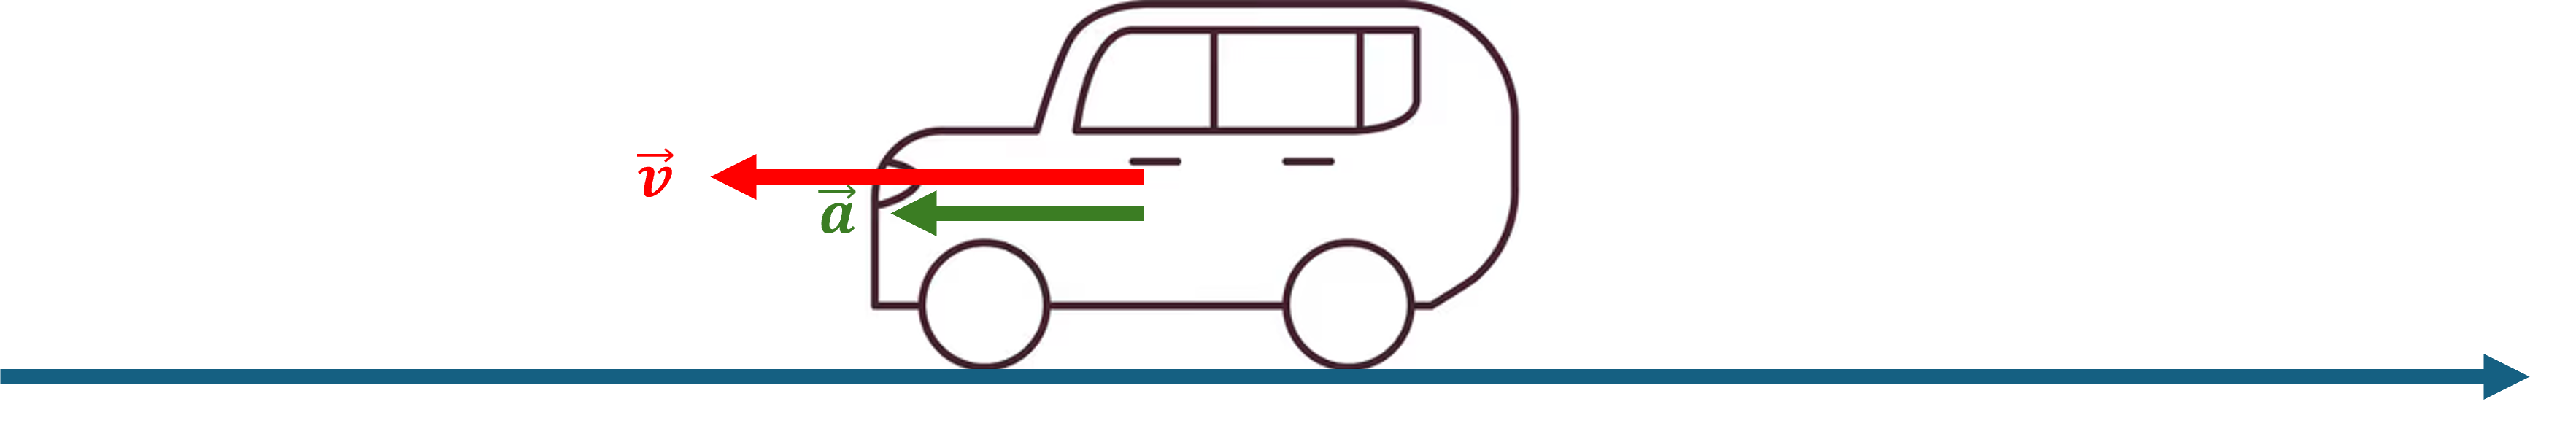
\includegraphics[width=0.9\linewidth]{Bilder/car_4.png}
\end{center}

\begin{parts}
  \part[2] Beschreibe in Worten, was mit dem Auto passiert.
  \Antwortraum{2}
  \begin{solution}
  Die Achse zeigt wieder nach rechts, die positive Richtung ist also
  rechts. $v$ und $a$ zeigen beide nach links, also gilt $v<0$ und $a<0$.
  Weil $v$ und $a$ dasselbe Vorzeichen haben, wird das Auto schneller,
  sichtbar bewegt es sich dabei nach links.
  \end{solution}

  \part[2] Skizziere das $s$-$t$-Diagramm.
  \begin{center}
  \begin{tikzpicture}[scale=0.6]
    \draw[->] (-0.3,0) -- (5.5,0) node[right] {\scriptsize $t$};
    \draw[->] (0,-3.5) -- (0,3.5) node[above] {\scriptsize $s$};
  \end{tikzpicture}
  \end{center}
  \begin{solution}
  \begin{center}
  \begin{tikzpicture}[scale=0.6]
    \draw[->] (-0.3,0) -- (5.5,0) node[right] {\scriptsize $t$};
    \draw[->] (0,-3.5) -- (0,3.5) node[above] {\scriptsize $s$};
    \draw[thick,titleblue,domain=0:4,samples=30,smooth] plot (\x,{-0.5*\x-0.1*\x*\x});
  \end{tikzpicture}
  \end{center}
  Steigung bei $t=0$ negativ (weil $v<0$), und die Kurve wird immer
  steiler nach unten (weil $a<0$): dieselbe Grundform wie bei Bild 1,
  nur an der $t$-Achse gespiegelt, weil hier $v$ und $a$ beide negativ
  statt beide positiv sind.
  \end{solution}

  \part[2] Skizziere das $v$-$t$-Diagramm.
  \begin{center}
  \begin{tikzpicture}[scale=0.6]
    \draw[->] (-0.3,0) -- (5.5,0) node[right] {\scriptsize $t$};
    \draw[->] (0,-3.5) -- (0,3.5) node[above] {\scriptsize $v$};
  \end{tikzpicture}
  \end{center}
  \begin{solution}
  \begin{center}
  \begin{tikzpicture}[scale=0.6]
    \draw[->] (-0.3,0) -- (5.5,0) node[right] {\scriptsize $t$};
    \draw[->] (0,-3.5) -- (0,3.5) node[above] {\scriptsize $v$};
    \draw[thick,titleblue] (0,-0.8) -- (4,-2.8);
  \end{tikzpicture}
  \end{center}
  Gerade mit negativem Achsenabschnitt (weil $v(0)<0$) und negativer
  Steigung (weil $a<0$).
  \end{solution}
\end{parts}
\end{taskbox}
\end{questions}

\begin{questions}
\setcounter{question}{11}
\begin{taskbox}[Übung: Schnelle Fahrzeuge]
Dieselbe Grundüberlegung wie oben, jetzt für zwei Fahrzeuge, die bereits
mit hoher Geschwindigkeit unterwegs sind (grosser $v$-Pfeil): Auch bei
grossem $v$ entscheidet weiterhin nur das Vorzeichen von $a$ relativ zu
$v$, ob das Auto schneller oder langsamer wird.

\question[2]
\begin{center}
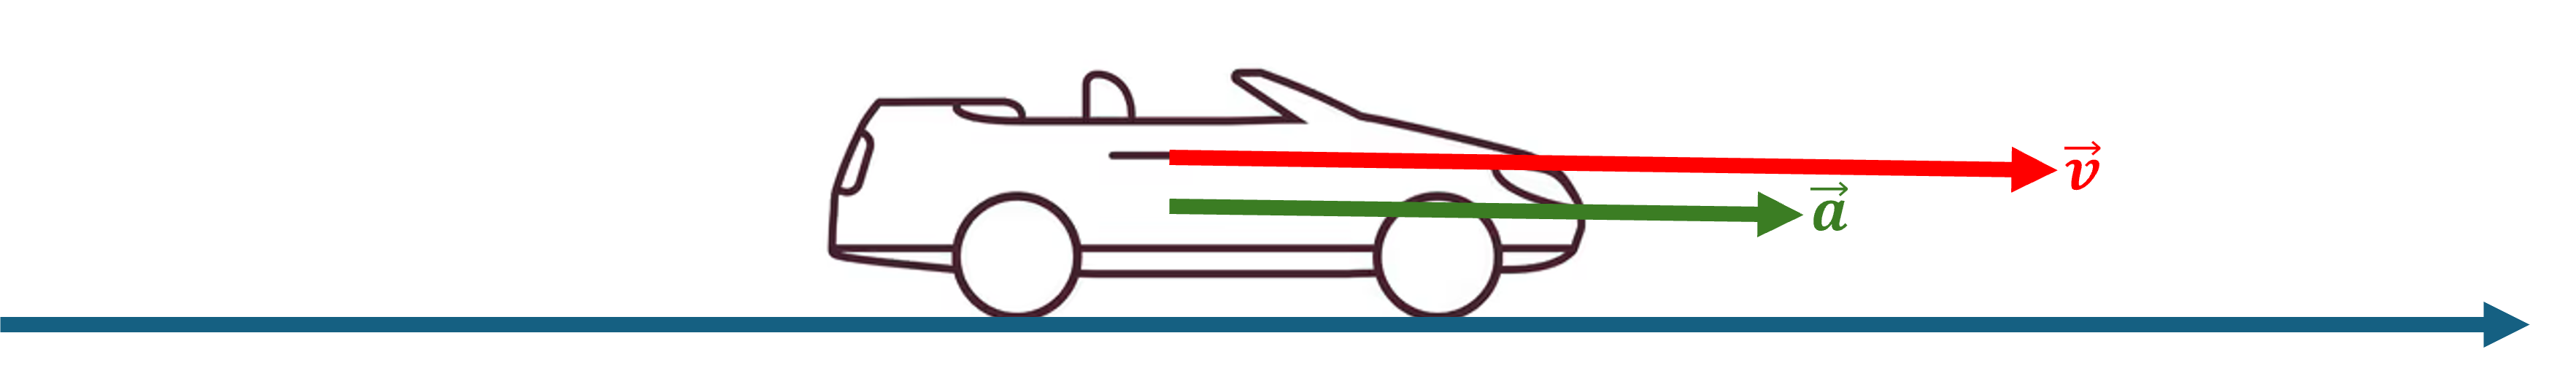
\includegraphics[width=0.9\linewidth]{Bilder/car_fast_1.png}
\end{center}
Beschreibe in Worten, was mit dem Auto passiert.
\Antwortraum{2}
\begin{solution}
Die Achse zeigt nach rechts, die positive Richtung ist also rechts.
$v$ und $a$ zeigen beide nach rechts, also gilt $v>0$ und $a>0$. Das
Auto ist bereits sehr schnell in positiver Richtung unterwegs und wird
wegen des gleichen Vorzeichens noch schneller: genau dieselbe Regel wie
bei kleinem $v$, ein grosses $v$ ändert daran nichts.
\end{solution}

\needspace{10\baselineskip}
\question[6]
\begin{center}
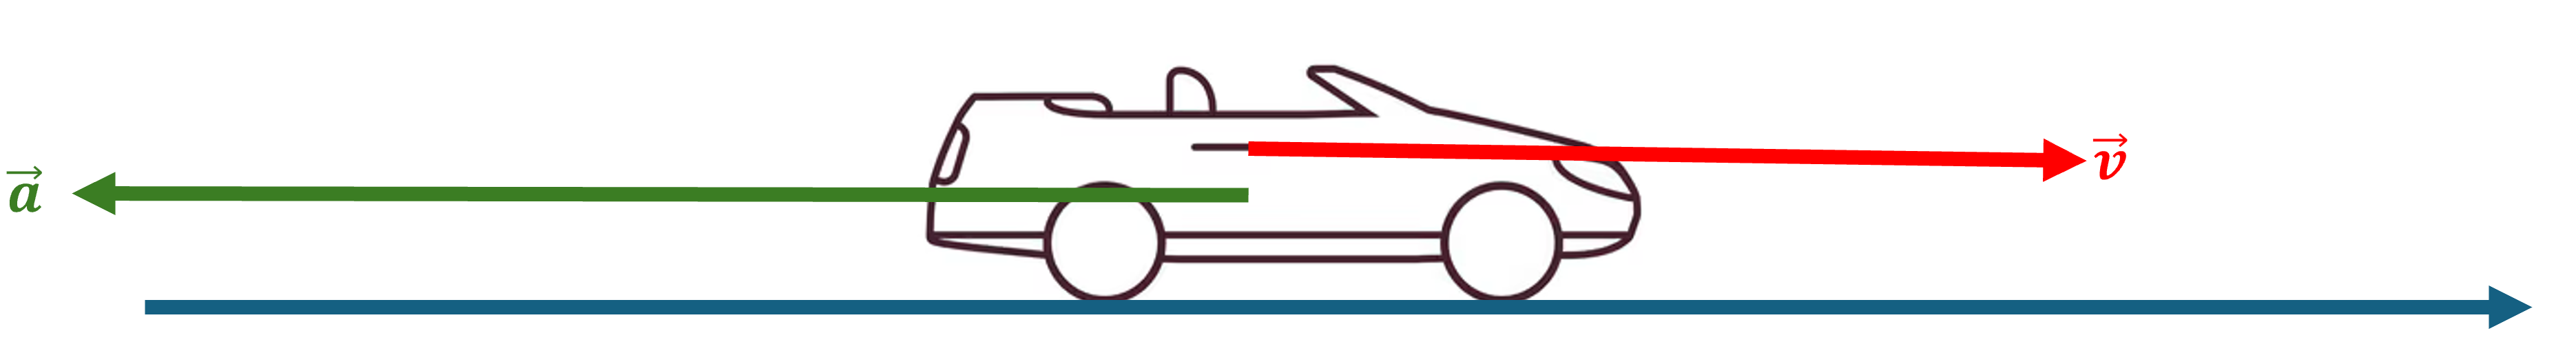
\includegraphics[width=0.9\linewidth]{Bilder/car_fast_2.png}
\end{center}

\begin{parts}
  \part[2] Beschreibe in Worten, was mit dem Auto passiert.
  \Antwortraum{2}
  \begin{solution}
  Die Achse zeigt nach rechts, die positive Richtung ist also rechts.
  $v$ zeigt nach rechts, also gilt $v>0$. $a$ zeigt nach links, also gilt
  $a<0$. Das Auto ist sehr schnell in positiver Richtung unterwegs, wird
  aber wegen des entgegengesetzten Vorzeichens stark abgebremst, es
  verzögert kräftig.
  \end{solution}

  \part[2] Skizziere das $s$-$t$-Diagramm.
  \begin{center}
  \begin{tikzpicture}[scale=0.6]
    \draw[->] (-0.3,0) -- (5.5,0) node[right] {\scriptsize $t$};
    \draw[->] (0,-1) -- (0,5) node[above] {\scriptsize $s$};
  \end{tikzpicture}
  \end{center}
  \begin{solution}
  \begin{center}
  \begin{tikzpicture}[scale=0.6]
    \draw[->] (-0.3,0) -- (5.5,0) node[right] {\scriptsize $t$};
    \draw[->] (0,-1) -- (0,5) node[above] {\scriptsize $s$};
    \draw[thick,titleblue,domain=0:4,samples=30,smooth] plot (\x,{0.9*\x-0.09*\x*\x});
  \end{tikzpicture}
  \end{center}
  Steigung bei $t=0$ stark positiv (weil $v(0)$ gross ist), die Kurve
  flacht aber deutlich ab (weil $a<0$ betragsmässig gross ist und der
  Geschwindigkeit stark entgegenwirkt).
  \end{solution}

  \part[2] Skizziere das $v$-$t$-Diagramm.
  \begin{center}
  \begin{tikzpicture}[scale=0.6]
    \draw[->] (-0.3,0) -- (5.5,0) node[right] {\scriptsize $t$};
    \draw[->] (0,-1) -- (0,5) node[above] {\scriptsize $v$};
  \end{tikzpicture}
  \end{center}
  \begin{solution}
  \begin{center}
  \begin{tikzpicture}[scale=0.6]
    \draw[->] (-0.3,0) -- (5.5,0) node[right] {\scriptsize $t$};
    \draw[->] (0,-1) -- (0,5) node[above] {\scriptsize $v$};
    \draw[thick,titleblue] (0,4) -- (4,0.3);
  \end{tikzpicture}
  \end{center}
  Gerade mit grossem positivem Achsenabschnitt (weil $v(0)$ gross ist)
  und deutlich negativer Steigung (weil $a<0$ betragsmässig gross ist),
  sie nähert sich der $t$-Achse an, ohne sie im gezeichneten Bereich zu
  erreichen.
  \end{solution}
\end{parts}
\end{taskbox}
\end{questions}

\begin{questions}
\setcounter{question}{13}
\begin{taskbox}[Zusatzaufgabe: Ein Auto im Stadtverkehr]
\question[13] Das folgende Diagramm zeigt schematisch, wie sich die
Geschwindigkeit eines Autos beim Losfahren, Weiterfahren und Anhalten
verändert:

\begin{center}
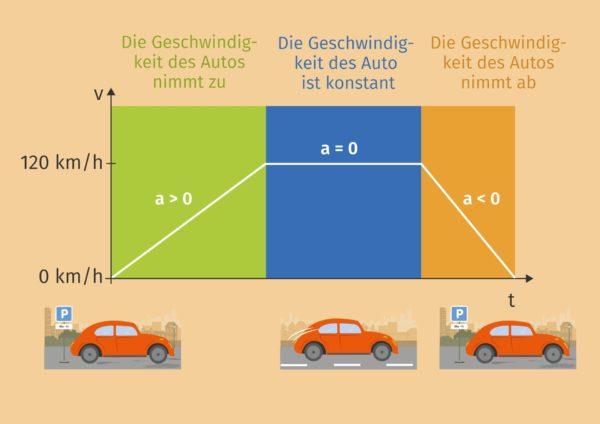
\includegraphics[width=0.7\linewidth]{Bilder/Auto_beschleunigung.jpg}\\
\footnotesize Schematische Darstellung ohne Zeitachse: Beschleunigen,
konstante Geschwindigkeit, Abbremsen.
\end{center}

Nimm für die folgenden Teilaufgaben konkrete Zeiten an: Das Auto
beschleunigt während $\SI{10}{\second}$ gleichmässig von
$\SI{0}{\kilo\meter\per\hour}$ auf $\SI{120}{\kilo\meter\per\hour}$
($\SI{120}{\kilo\meter\per\hour} : 3.6 \approx \SI{33.3}{\meter\per\second}$).
Danach fährt es $\SI{15}{\second}$ lang mit konstanter Geschwindigkeit
weiter. Anschliessend bremst es innerhalb von $\SI{6}{\second}$
gleichmässig bis zum Stillstand ab.

\begin{parts}
  \part[3] Das $v$-$t$-Diagramm oben zeigt bereits die Form der Bewegung.
  Skizziere qualitativ, ohne Zahlen, wie das zugehörige $a$-$t$-Diagramm
  für dieselbe Fahrt aussehen müsste. Orientiere dich an den Phasen
  $a>0$, $a=0$ und $a<0$ aus dem Bild oben.

  \begin{center}
  \begin{tikzpicture}[scale=0.6]
    \draw[->] (-0.3,0) -- (7.5,0) node[right] {\scriptsize $t$};
    \draw[->] (0,-2.5) -- (0,3) node[above] {\scriptsize $a$};
  \end{tikzpicture}
  \end{center}
  \begin{solution}
  \begin{center}
  \begin{tikzpicture}[scale=0.6]
    \draw[->] (-0.3,0) -- (7.5,0) node[right] {\scriptsize $t$};
    \draw[->] (0,-2.5) -- (0,3) node[above] {\scriptsize $a$};
    \draw[thick,titleblue] (0,1.5) -- (2,1.5);
    \draw[dashed,gray] (2,1.5) -- (2,0);
    \draw[thick,titleblue] (2,0) -- (5,0);
    \draw[dashed,gray] (5,0) -- (5,-2);
    \draw[thick,titleblue] (5,-2) -- (7,-2);
  \end{tikzpicture}
  \end{center}
  In der ersten Phase ist $a$ konstant positiv (Beschleunigen), in der
  zweiten Phase ist $a=0$ (konstante Geschwindigkeit), und in der
  dritten Phase ist $a$ konstant negativ (Abbremsen), betragsmässig
  grösser als in der ersten Phase, weil das Auto in kürzerer Zeit stärker
  bremst als es beschleunigt hat.
  \end{solution}

  \part[3] Skizziere qualitativ, ohne Zahlen, wie das zugehörige
  $s$-$t$-Diagramm für dieselbe Fahrt aussehen müsste.

  \begin{center}
  \begin{tikzpicture}[scale=0.6]
    \draw[->] (-0.3,0) -- (7.5,0) node[right] {\scriptsize $t$};
    \draw[->] (0,-0.3) -- (0,10.5) node[above] {\scriptsize $s$};
  \end{tikzpicture}
  \end{center}
  \begin{solution}
  \begin{center}
  \begin{tikzpicture}[scale=0.6]
    \draw[->] (-0.3,0) -- (7.5,0) node[right] {\scriptsize $t$};
    \draw[->] (0,-0.3) -- (0,10.5) node[above] {\scriptsize $s$};
    \draw[thick,titleblue,domain=0:2,samples=30,smooth] plot (\x,{0.5*\x*\x});
    \draw[thick,titleblue] (2,2) -- (5,8);
    \draw[thick,titleblue,domain=5:7,samples=30,smooth] plot (\x,{8+2*(\x-5)-0.5*(\x-5)*(\x-5)});
  \end{tikzpicture}
  \end{center}
  Im ersten Abschnitt (Beschleunigen) wird die Kurve immer steiler, im
  zweiten Abschnitt (konstante Geschwindigkeit) ist sie eine Gerade, und
  im dritten Abschnitt (Abbremsen) flacht sie wieder ab, bis sie
  waagrecht wird.
  \end{solution}

  % Verhindert, dass die Aufgabenstellung von Teilaufgabe (c) allein am
  % Seitenende steht, während ihr Antwortraum erst auf der Folgeseite
  % erscheint (analog zum \needspace an anderen Stellen im Dokument).
  \needspace{5\baselineskip}
  \part[2] Berechne die Beschleunigung während der ersten
  $\SI{10}{\second}$ (Losfahren).
  \Antwortraum{2}
  \begin{solution}
  $a_1 = \dfrac{\Delta v}{\Delta t} = \dfrac{\SI{33.3}{\meter\per\second}}{\SI{10}{\second}} \approx \SI{3.3}{\meter\per\second\squared}$.
  \end{solution}

  \part[2] Berechne die Beschleunigung während der letzten
  $\SI{6}{\second}$ (Abbremsen).
  \Antwortraum{2}
  \begin{solution}
  $a_3 = \dfrac{\Delta v}{\Delta t} = \dfrac{\SI{0}{\meter\per\second} - \SI{33.3}{\meter\per\second}}{\SI{6}{\second}} \approx -\SI{5.6}{\meter\per\second\squared}$.
  \end{solution}

  \part[3] Bestimme mithilfe von Flächenberechnungen (Rechteck und zwei
  Dreiecke, analog zum $v$-$t$-Diagramm oben) die gesamte während der
  Fahrt zurückgelegte Strecke.
  \Antwortraum{3}
  \begin{solution}
  Dreieck (Beschleunigen): $\tfrac12\cdot\SI{10}{\second}\cdot\SI{33.3}{\meter\per\second}
  \approx \SI{167}{\meter}$.\\
  Rechteck (konstant): $\SI{15}{\second}\cdot\SI{33.3}{\meter\per\second}
  \approx \SI{500}{\meter}$.\\
  Dreieck (Abbremsen): $\tfrac12\cdot\SI{6}{\second}\cdot\SI{33.3}{\meter\per\second}
  \approx \SI{100}{\meter}$.\\
  Gesamt: $\approx \SI{167}{\meter} + \SI{500}{\meter} + \SI{100}{\meter}
  = \SI{767}{\meter}$.
  \end{solution}
\end{parts}
\end{taskbox}
\end{questions}

% =============================================================================
% Vertiefung zum Schluss: Durchschnitts- vs. Momentanbeschleunigung
% (LZ2/LZ3). Die allgemeine Formel a=Delta v/Delta t wurde bereits ganz am
% Anfang eingeführt (siehe formelbox oben) und in den Aufgaben mehrfach
% angewendet -- hier deshalb nur noch die Unterscheidung Sekante/Tangente,
% keine erneute Formelherleitung.
% =============================================================================
\begin{theoriebox}[Durchschnitts- und Momentanbeschleunigung]
Wie du in den Aufgaben oben bereits mit der Formel $a=\Delta v/\Delta t$
berechnet hast: Die Beschleunigung lässt sich im $v$-$t$-Diagramm als
Steigung ablesen, genau wie die Geschwindigkeit im $s$-$t$-Diagramm.

Wird $a$ zwischen zwei Zeitpunkten $t_1$ und $t_2$ berechnet, erhält man
genau genommen die \textbf{\emph{Durchschnittsbeschleunigung}} $\bar a$
zwischen diesen beiden Zeitpunkten, die Sekantensteigung im
$v$-$t$-Diagramm.

Will man wissen, wie stark ein Objekt zu einem einzelnen Zeitpunkt $t_0$
beschleunigt, braucht man stattdessen die
\textbf{\emph{Momentanbeschleunigung}} $a(t_0)$: Ist der Graph im
$v$-$t$-Diagramm eine Gerade, ist die Momentanbeschleunigung überall
gleich der Durchschnittsbeschleunigung. Ist der Graph gekrümmt, zeichnet
man an der Stelle $t_0$ die \textbf{\emph{Tangente}} und liest deren
Steigung ab, genau wie bei der Momentangeschwindigkeit im
$s$-$t$-Diagramm.

\begin{center}
\begin{tikzpicture}[scale=0.9]
  \draw[->] (-0.3,0) -- (6.7,0) node[right] {\scriptsize $t$};
  \draw[->] (0,-0.3) -- (0,6) node[above] {\scriptsize $v$};
  \draw[thick,titleblue,domain=0:6,samples=60,smooth] plot (\x,{0.15*\x*\x});
  \draw[thick,accentorange] (1,0.15) -- (5,3.75) node[right] {\scriptsize Sekante: $\bar a$};
  \draw[thick,accentpurple] (2.5,0.6) -- (5.5,4.2) node[right] {\scriptsize Tangente: $a(t_0)$};
  \filldraw[black] (1,0.15) circle (1.6pt);
  \filldraw[black] (5,3.75) circle (1.6pt);
  \filldraw[black] (4,2.4) circle (1.6pt);
  \draw (1,0.05) -- (1,-0.05) node[below] {\scriptsize $t_1$};
  \draw (4,0.05) -- (4,-0.05) node[below] {\scriptsize $t_0$};
  \draw (5,0.05) -- (5,-0.05) node[below] {\scriptsize $t_2$};
  \draw (0.08,0.15) -- (-0.08,0.15) node[left] {\scriptsize 0.15};
  \draw (0.08,3.75) -- (-0.08,3.75) node[left] {\scriptsize 3.75};
\end{tikzpicture}
\end{center}

Auch hier gilt: Die Momentanbeschleunigung ist der Grenzwert der
Durchschnittsbeschleunigung für $\Delta t \to 0$.
\end{theoriebox}

\begin{questions}
\setcounter{question}{14}
\begin{taskbox}[Übung: Durchschnitts- und Momentanbeschleunigung ablesen]
\question[4] Im Diagramm oben gilt $v(t_1)=\SI{0.15}{\meter\per\second}$
bei $t_1=\SI{1}{\second}$ und $v(t_2)=\SI{3.75}{\meter\per\second}$ bei
$t_2=\SI{5}{\second}$ (Sekante, orange).

\begin{parts}
  \part[2] Berechne die Durchschnittsbeschleunigung $\bar a$ zwischen
  $t_1$ und $t_2$.
  \Antwortraum{2}
  \begin{solution}
  \[
    \bar a = \frac{v(t_2)-v(t_1)}{t_2-t_1} =
    \frac{\SI{3.75}{\meter\per\second} - \SI{0.15}{\meter\per\second}}{\SI{5}{\second}-\SI{1}{\second}} =
    \frac{\SI{3.6}{\meter\per\second}}{\SI{4}{\second}} = \SI{0.9}{\meter\per\second\squared}.
  \]
  \end{solution}

  \part[2] Ist die Momentanbeschleunigung $a(t_0)$ bei $t_0$ (violette
  Tangente) grösser oder kleiner als $\bar a$? Begründe mit der Steigung
  der beiden Linien im Diagramm, ohne sie zu berechnen.
  \Antwortraum{2}
  \begin{solution}
  Die Tangente bei $t_0$ ist im Diagramm sichtbar steiler als die
  Sekante, also gilt $a(t_0) > \bar a$: Die Momentanbeschleunigung an
  diesem Zeitpunkt ist grösser als die Durchschnittsbeschleunigung über
  das ganze Intervall $[t_1,t_2]$, weil die Kurve gegen $t_2$ hin immer
  steiler wird.
  \end{solution}
\end{parts}
\end{taskbox}
\end{questions}

\end{document}
